 \documentclass[12pt, dvipdfmx]{beamer}

\renewcommand{\kanjifamilydefault}{\gtdefault}
%%%%%%%%%%%  package  %%%%%%%%%%%
\usepackage{bxdpx-beamer}% dvipdfmxなので必要
\usepackage{pxjahyper}% 日本語で'しおり'したい

% \hypersetup{colorlinks=true, linkcolor=black, citecolor=blue}

\usepackage{amssymb,amsmath,ascmac}

\usepackage{multirow}
\usepackage{bm}

\graphicspath{{../../_Figures//}{../../_Figures/Rheology/}}

\usepackage{tikz}
\usepackage{xparse}

\usepackage{multimedia}

\usetikzlibrary{shapes,arrows}
%% define fancy arrow. \tikzfancyarrow[<option>]{<text>}. ex: \tikzfancyarrow[fill=red!5]{hoge}
\tikzset{arrowstyle/.style n args={2}{inner ysep=0.1ex, inner xsep=0.5em, minimum height=2em, draw=#2, fill=black!20, font=\sffamily\bfseries, single arrow, single arrow head extend=0.4em, #1,}}
\NewDocumentCommand{\tikzfancyarrow}{O{fill=black!20} O{none}  m}{
\tikz[baseline=-0.5ex]\node [arrowstyle={#1}{#2}] {#3 \mathstrut};}

%目次スライド
\AtBeginSection[]{
  \frame{\tableofcontents[currentsection]}
}

%アペンディックスのページ番号除去
\newcommand{\backupbegin}{
   \newcounter{framenumberappendix}
   \setcounter{framenumberappendix}{\value{framenumber}}
}
\newcommand{\backupend}{
   \addtocounter{framenumberappendix}{-\value{framenumber}}
   \addtocounter{framenumber}{\value{framenumberappendix}} 
}

\newcommand{\rmd}{\mathrm{d}}
\newcommand{\dd}[1]{\dfrac{\mathrm{d} #1}{\mathrm{d} x}}

%%%%%%%%%%%  theme  %%%%%%%%%%%
\usetheme{Copenhagen}
% \usetheme{Metropolis}
% \usetheme{CambridgeUS}
% \usetheme{Berlin}

%%%%%%%%%%%  inner theme  %%%%%%%%%%%
% \useinnertheme{default}

% %%%%%%%%%%%  outer theme  %%%%%%%%%%%
\useoutertheme{default}
% \useoutertheme{infolines}

%%%%%%%%%%%  color theme  %%%%%%%%%%%
%\usecolortheme{structure}

%%%%%%%%%%%  font theme  %%%%%%%%%%%
\usefonttheme{professionalfonts}
%\usefonttheme{default}

%%%%%%%%%%%  degree of transparency  %%%%%%%%%%%
%\setbeamercovered{transparent=30}

% \setbeamertemplate{items}[default]

%%%%%%%%%%%  numbering  %%%%%%%%%%%
% \setbeamertemplate{numbered}
\setbeamertemplate{navigation symbols}{}
\setbeamertemplate{footline}[frame number]


\title
[複雑な事象について]
{複雑な事象について}
\author[東亞合成 佐々木]{佐々木 裕\thanks{hiroshi\_sasaki@mail.toagosei.co.jp}}
\institute[東亞合成]{東亞合成株式会社}
\date{}

\begin{document}

%%%%%
% 1 P
%%%%%
\maketitle

%%%%%
% 2 P
%%%%%
%% 目次 (必要なければ省略)
\begin{frame}
\frametitle{Outline}
\tableofcontents
\end{frame}

\begin{frame}
	\frametitle{この章でのお話}
		この章では、「複雑な事象」についての議論を進めていきます。

		以前にも述べましたように、実際の事象は非常に複雑なものとなっています。
		この複雑な現象を考察するために、最もシンプルなニュートン流体の流動を表すモデルを振り返った上で、
		それとの相違という形で考えていきましょう。

	% 具体的に列記すると、以下のような事項となります。
	\begin{itemize}
		\item 流れるということについて、もう少し。
		% \begin{itemize}
		% 	\item 
		% \end{itemize} 
		\item 非ニュートン流体とは?
		% \begin{itemize}
		% 	\item 
		% \end{itemize} 
		\item 実事象についても少しだけ考えましょう。
		% \begin{itemize}
		% 	\item 
		% \end{itemize}
	\end{itemize}
\end{frame}

\section{流れるということについて、もう少し}

\subsection{ニュートン流体を見直しましょう}
\begin{frame}
    \frametitle{ニュートンの法則}
		\begin{columns}[T, onlytextwidth]
			\column{.48\linewidth}
				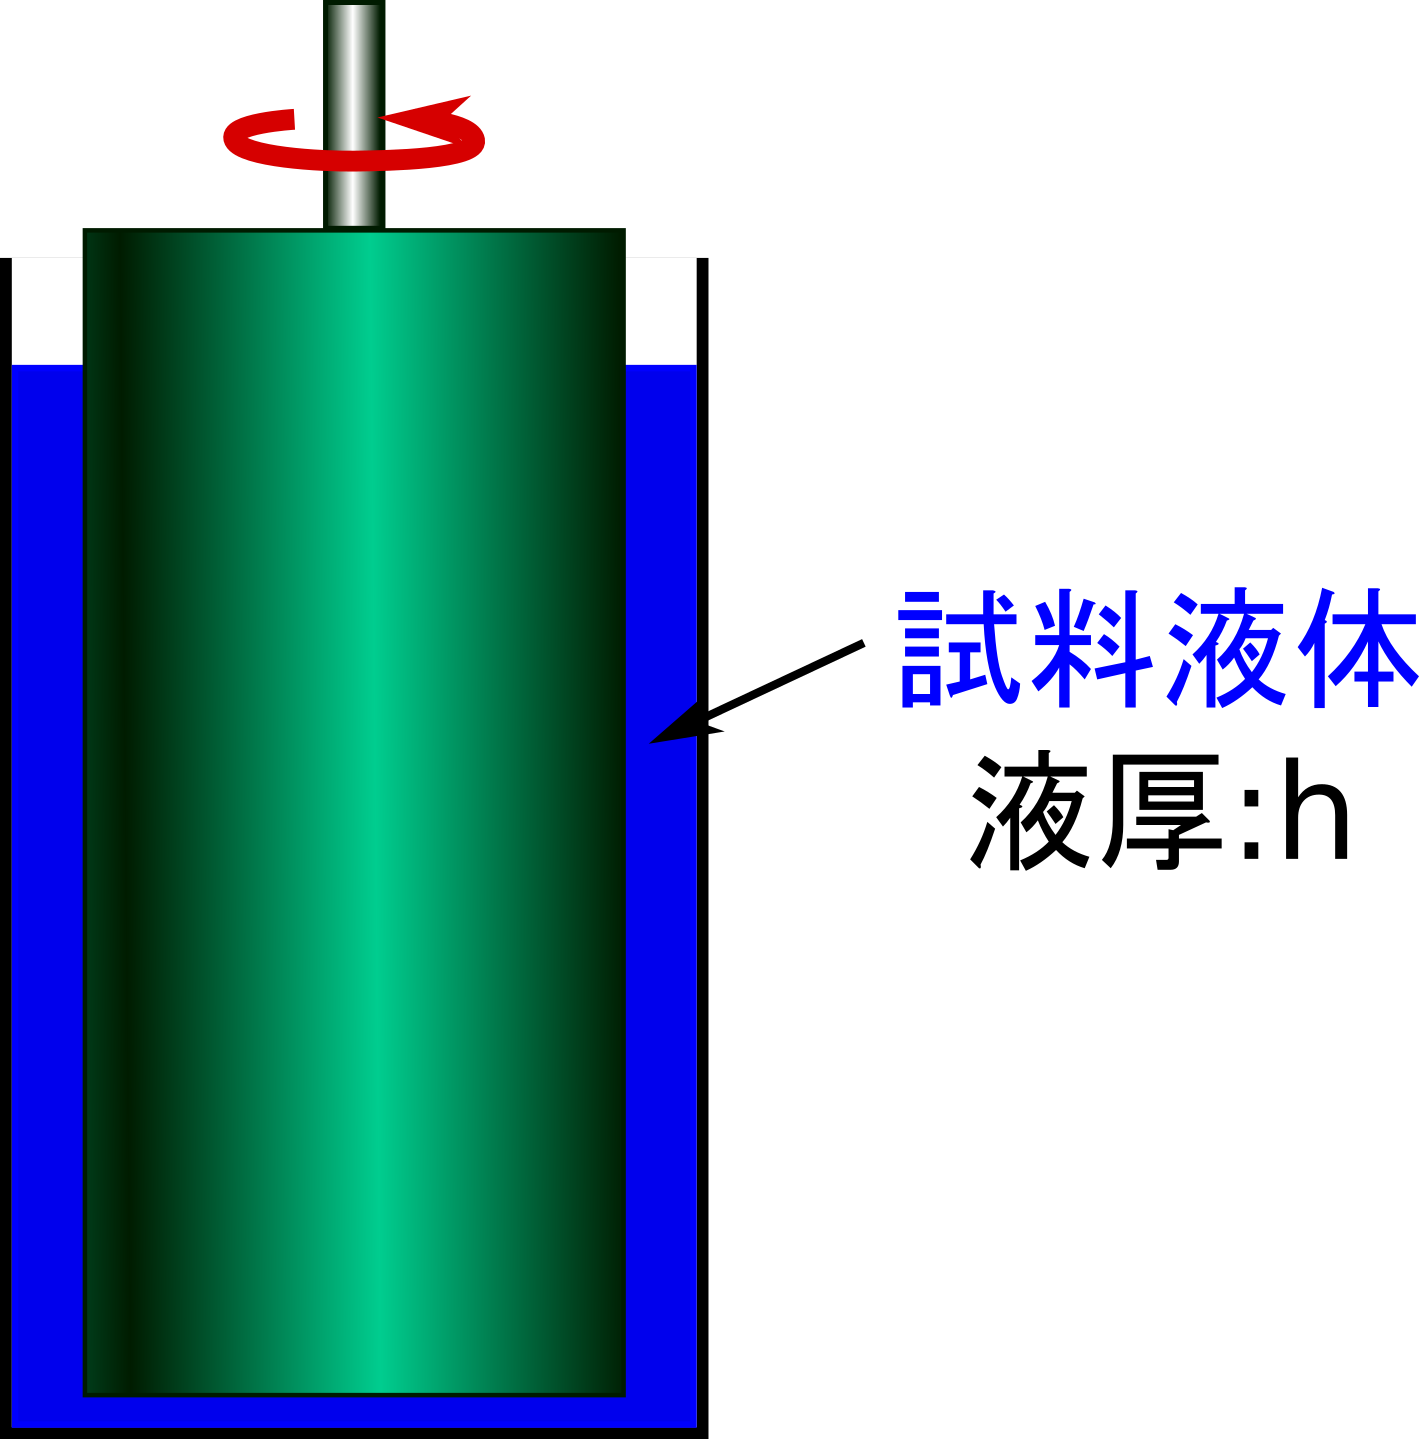
\includegraphics[width=.65\textwidth]{nijyu_entou.png}
			\column{.48\linewidth}
				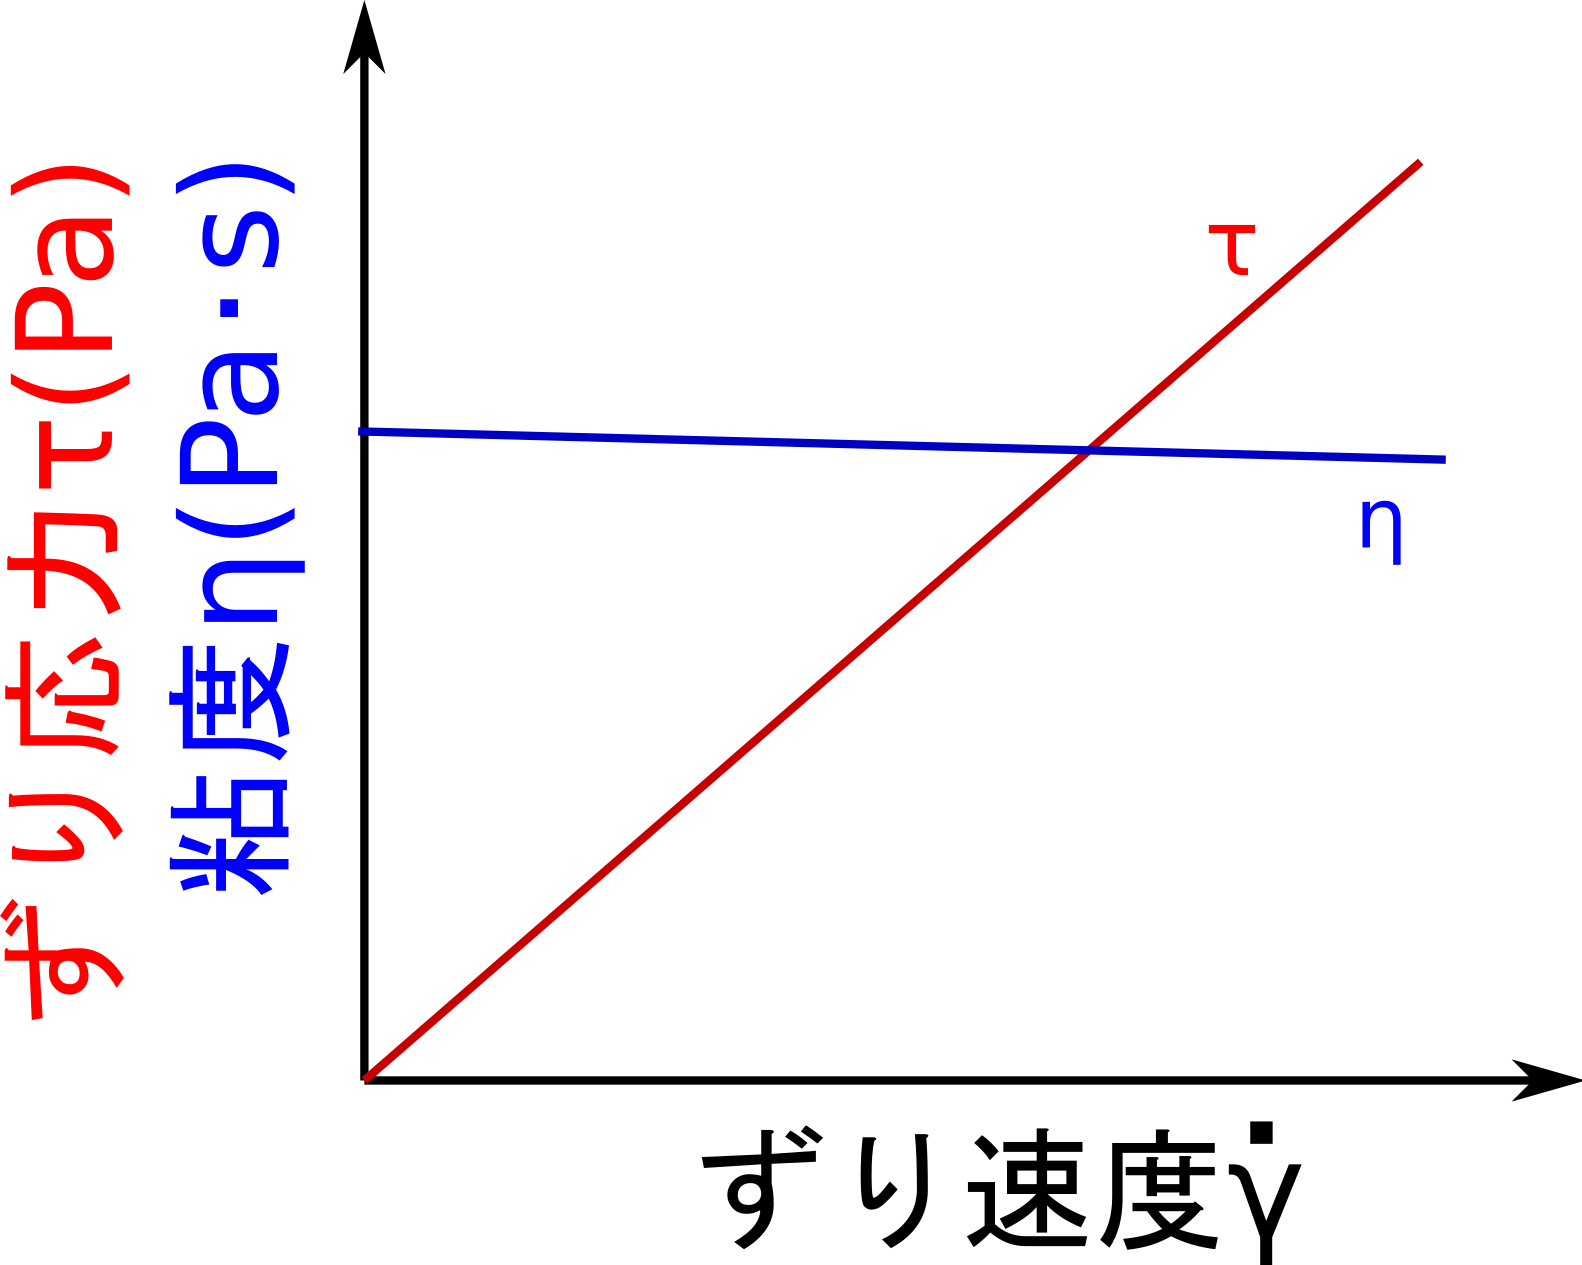
\includegraphics[width=.85\textwidth]{newtonian.png}
		\end{columns}
		\begin{exampleblock}{ニュートンの法則}
			\vspace{-5mm}
			\begin{align*}
				\text{せん断応力} &= \text{粘度} \times \text{せん断速度} \notag \\
				\tau = \eta \dot{\gamma}
			\end{align*}
			\vspace{-8mm}
			\begin{itemize}
				\item ずり応力はずり速度に比例。
				\item 比例定数の粘度は、ずり速度によらずに一定。
			\end{itemize}
		\end{exampleblock}
\end{frame}

\subsection{流動を表すモデル}
\begin{frame}
	\frametitle{液体の流動を表すモデル}
	\begin{exampleblock}{水面に板を浮かべたモデル}
		\begin{columns}[T, onlytextwidth]
			\column{.65\linewidth}
				\begin{itemize}
					\item 水深方向に n+1 層に分割
						\begin{itemize}
							\item 水面の板との境目を0
							\item 水底との境目を n 
						\end{itemize}
						\item 液体の内部では、
						\begin{itemize}
							\item 水深に応じて流れる速度の分布
							\item 最も単純な状態:\\速度勾配が一定
						\end{itemize}
				\end{itemize}
			\column{.32\linewidth}
				\begin{center}
					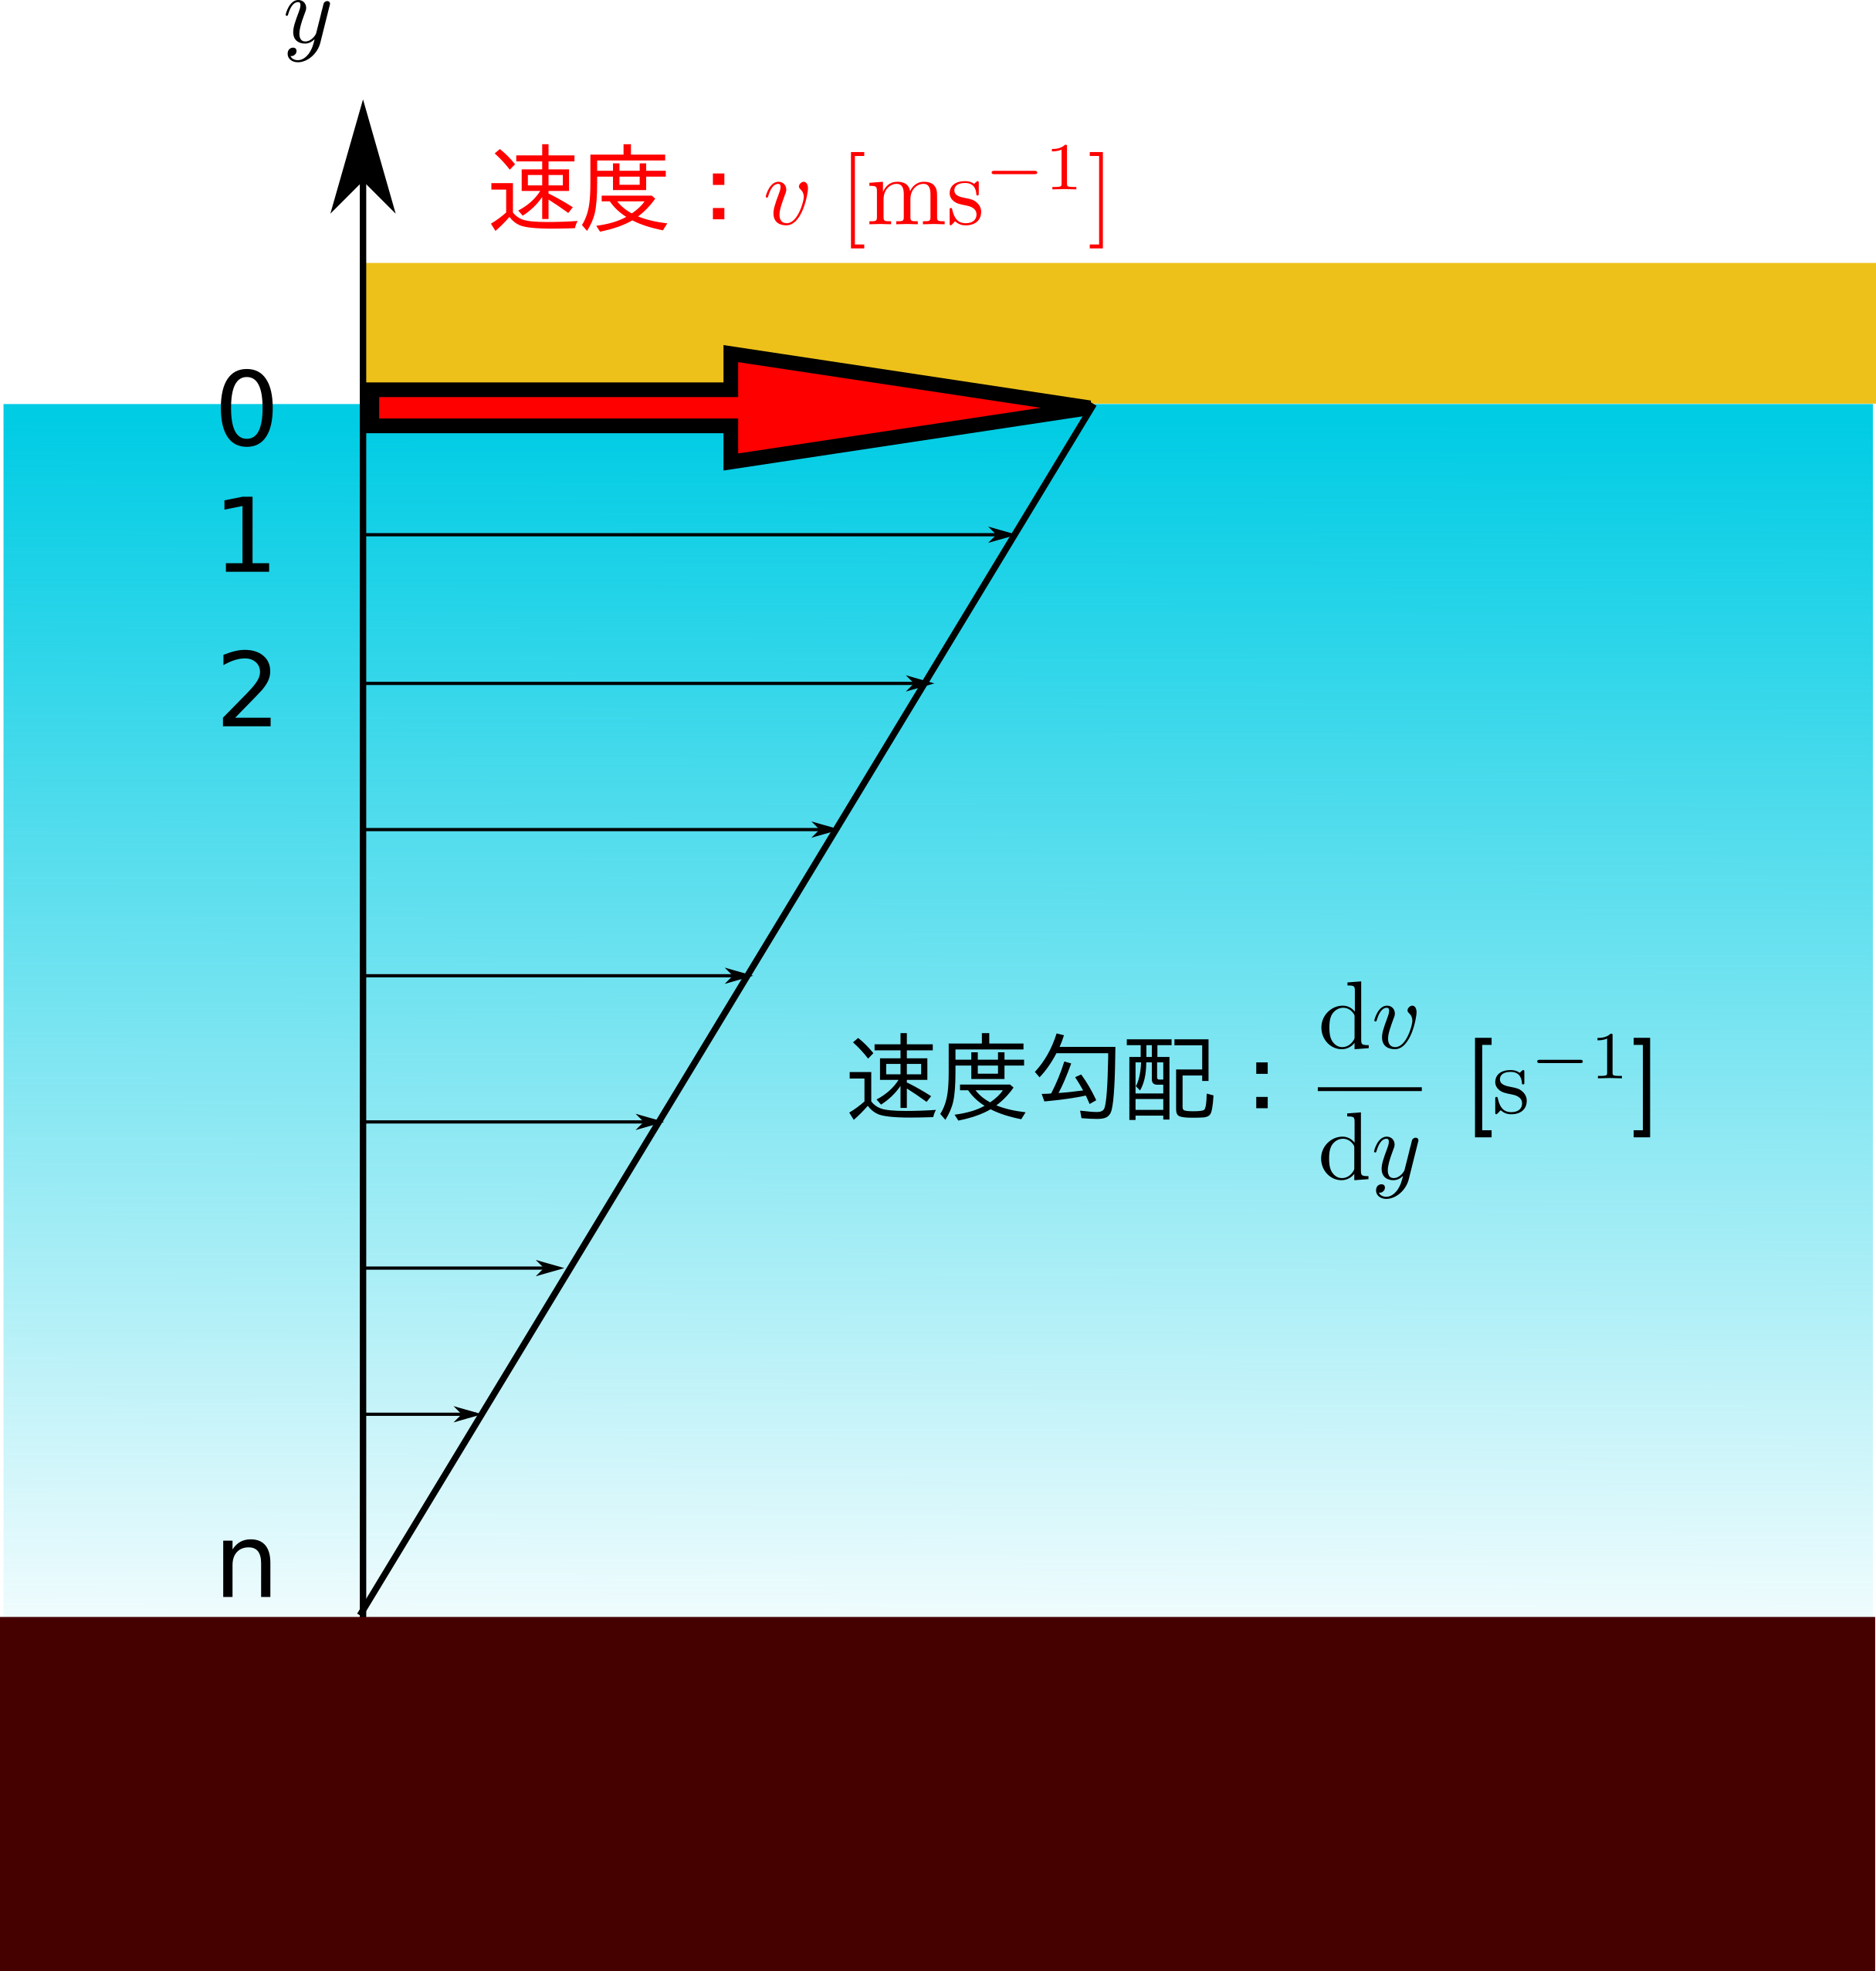
\includegraphics[width=.9\textwidth]{shear_3.png}
				\end{center}
		\end{columns}
	\end{exampleblock}
	\begin{block}{液体を考えるときに重要な事項}
		\begin{itemize}
			\item \textcolor{red}{固体と接している液体はその相対的な移動速度が同じ}
			\begin{itemize}
				\item 移動する板と接している\alert{層 0 は板と同じ速度 $v$ で流れ、}
				\item \textcolor{red}{地面に接している層 $n$ は流れない。}
			\end{itemize}
		\end{itemize}
	\end{block}
\end{frame}

\begin{frame}
	\frametitle{液体の流動について}
		\begin{itemize}
			\item 評価の対象である液体の内部では、
			\begin{itemize}
				\item 水深に応じて、流れる速度の分布が生じる
			\end{itemize}
			\item 液体の流れる速度は、
			\begin{itemize}
				\item 水深 $y$ の関数として $v(y)$
				\item 速度勾配と呼ばれ、その単位は $[\mathrm{s^{-1}}]$
			\end{itemize}
		\end{itemize}
		\begin{screen}
			速度勾配は、せん断変形を記述する無次元量であるせん断ひずみ $\gamma$ の時間変化(微分)$\Leftrightarrow$ せん断速度
			\begin{align*}
				\dfrac{\mathrm{d} v}{\mathrm{d} y} =\dot{\gamma} [s^{-1}]
			\end{align*}
		\end{screen}
\end{frame}

\begin{frame}
	\frametitle{液体の力学モデル}
	\vspace{-3mm}
		\begin{columns}[c, onlytextwidth]
			\column{.48\linewidth}
				\begin{itemize}
					\item せん断速度$\dot{\gamma}$ に比例し、
					\item せん断応力 $\tau$ が生じ、
					\item 比例定数が粘度 $\eta$
				\end{itemize}
				\vspace{-2mm}
				\begin{align*}
					\tau = \eta \dot{\gamma}
				\end{align*}
				\vspace{-6mm}
				\begin{screen}
					上記の比例関係が成立する液体がニュートン流体
				\end{screen}
			\column{.48\linewidth}
				\begin{center}
					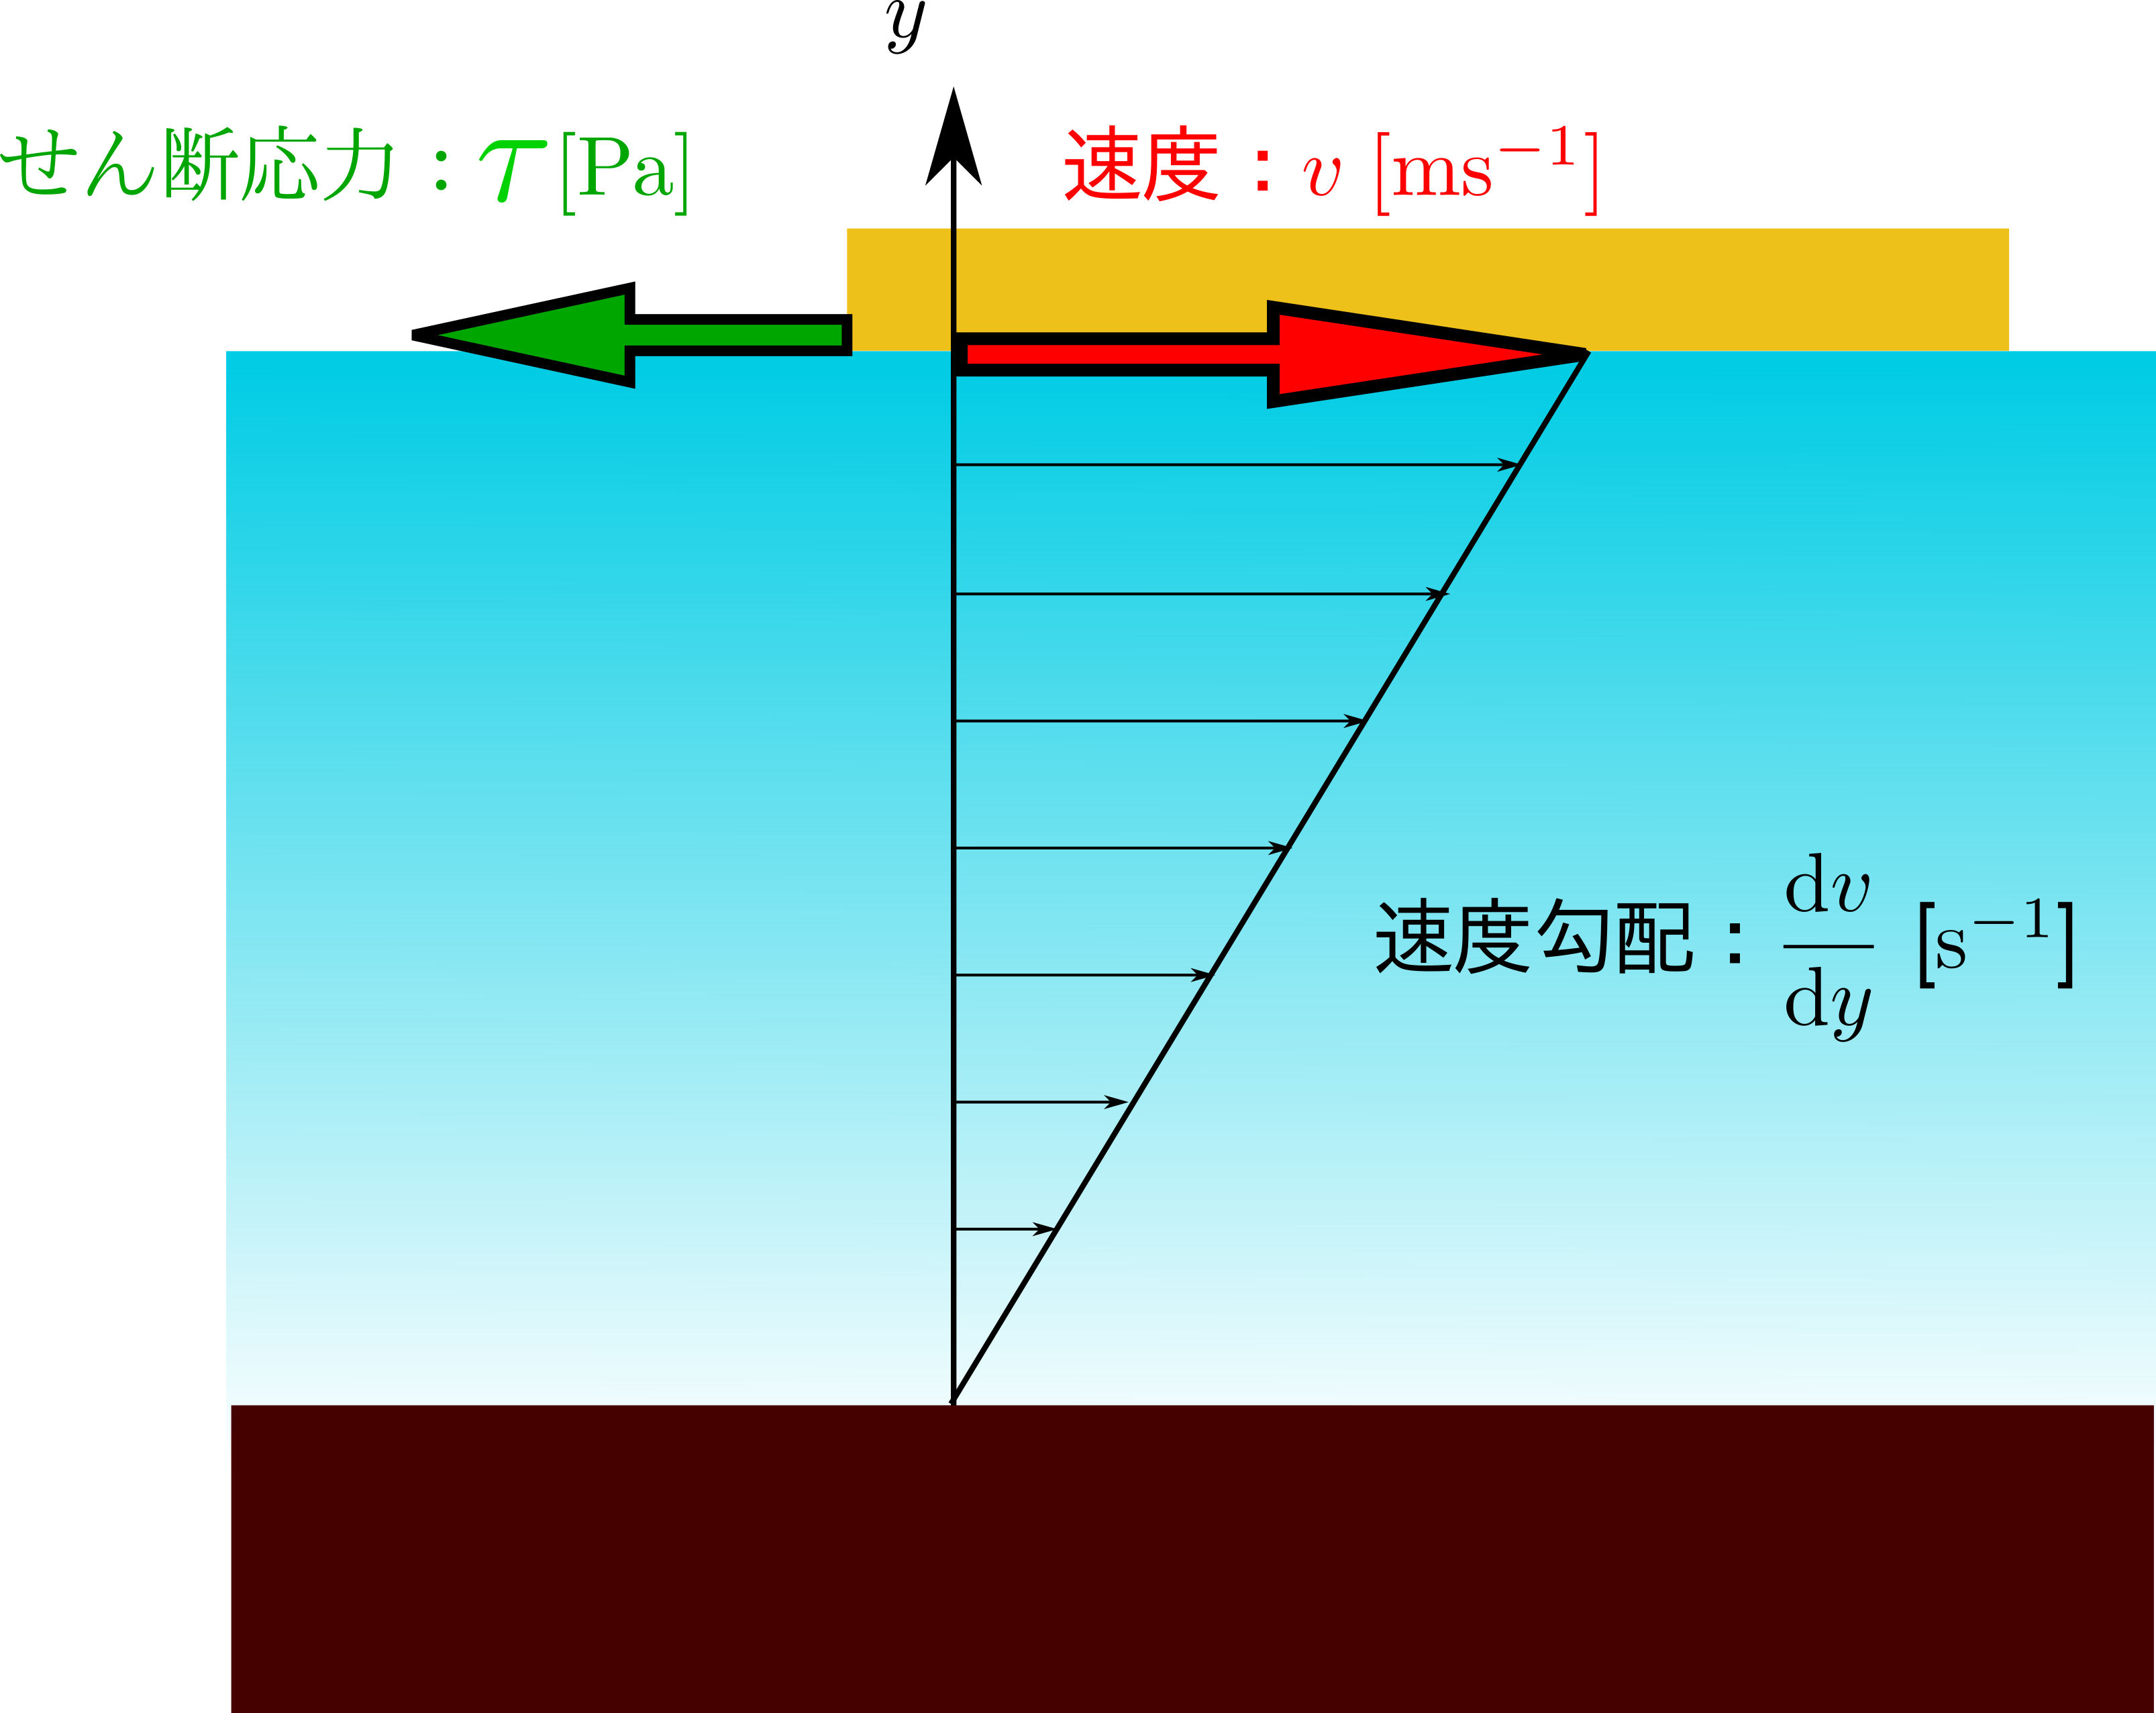
\includegraphics[width=\textwidth]{shear_4.png}
				\end{center}
		\end{columns}
		\begin{alertblock}{注意点}
			\begin{itemize}
				\item 速度勾配に従って、各層ごとにせん断応力が発生
				\item その値は、\alert{局所的なせん断速度に比例して変化。}
				\item 逆に言えば、\alert{せん断速度によらずに粘度が一定。}
			\end{itemize}
		\end{alertblock}
\end{frame}

\subsection{局所的な応力と粘度}
\begin{frame}
	\frametitle{液体の応力とは?(再掲)}
		\begin{itemize}
			\item マクロな変形(例えば、ずり変形)を付与
			\begin{itemize}
				\item ミクロにも粒子近傍の並び方が変化
			\end{itemize}
			\item 一粒子に着目すると、
			\begin{itemize}
				\item その粒子を取り巻く周りの粒子とのポテンシャル場が変化して、\textcolor{red}{「歪んだかご」}
				\item 「歪んだかご」の中で、\textcolor{red}{居心地が悪くなる。}
				\item その結果として\textcolor{red}{局所的な応力が発現}
			\end{itemize}
			\item その積分値として、マクロな応力
			\begin{itemize}
				\item 「歪んだかご」からの\alert{脱出 $\Leftrightarrow$ ミクロな応力が消失 }
				\item マクロにも\alert{流動}
			\end{itemize}
		\end{itemize}
		\vspace{3mm}
		\begin{center}
			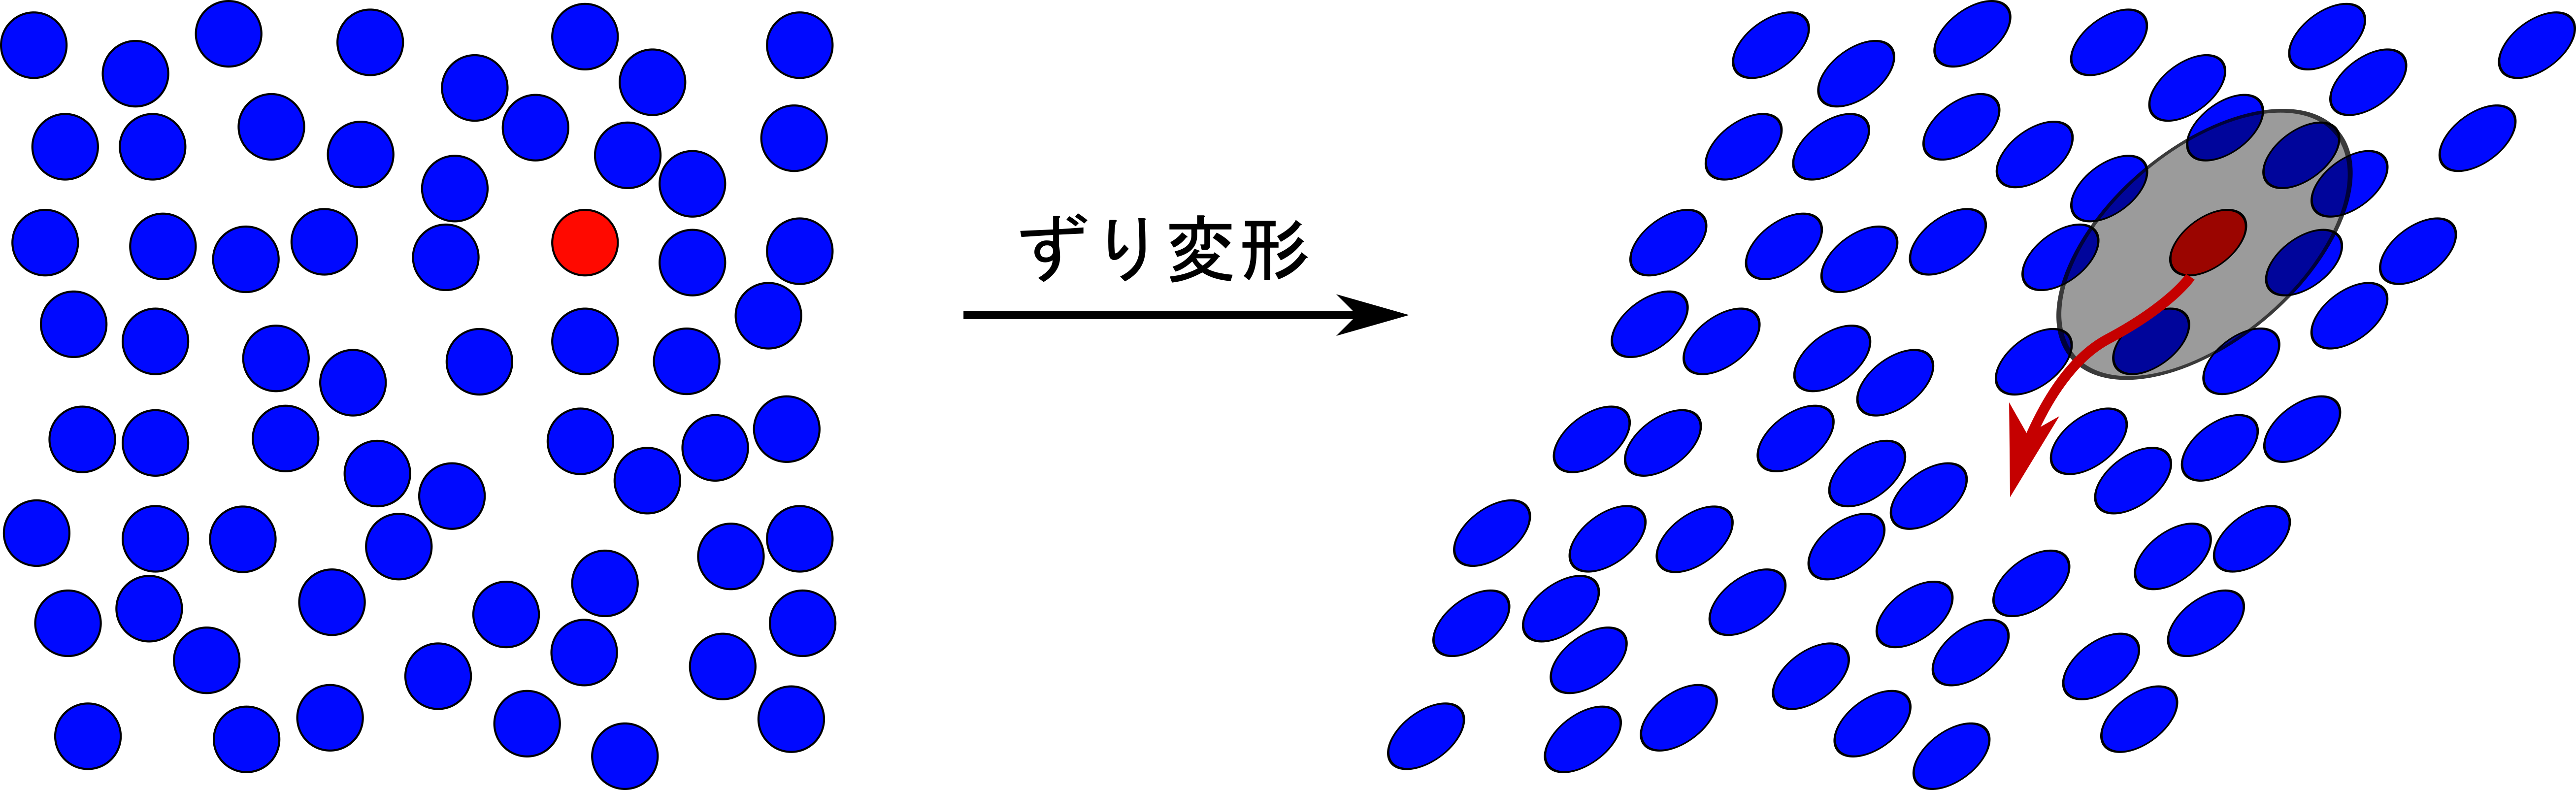
\includegraphics[width=.6\textwidth]{liquid_flow.png}
		\end{center}
\end{frame}

\begin{frame}
	\frametitle{粘度が「せん断速度」に依存しない理由}
		\vspace{-3mm}
		\begin{columns}[T, onlytextwidth]
			\column{.48\linewidth}
				\begin{block}{せん断応力の由来}
					\begin{itemize}
						\item 仮想的な面で生じる\\せん断応力の由来は、
						\begin{itemize}
							\item \alert{面を通しての粒子の相互作用}に起因
							\item 相対的な速度差に、比例する
						\end{itemize}
						\item この相互作用は、
						\begin{itemize}
							\item 「歪んだかご」からの脱出頻度にも比例
							\item 多体の相互作用が、「居心地の悪さ」
						\end{itemize}
					\end{itemize}
				\end{block}
			\column{.48\linewidth}
				\vspace{3mm}
				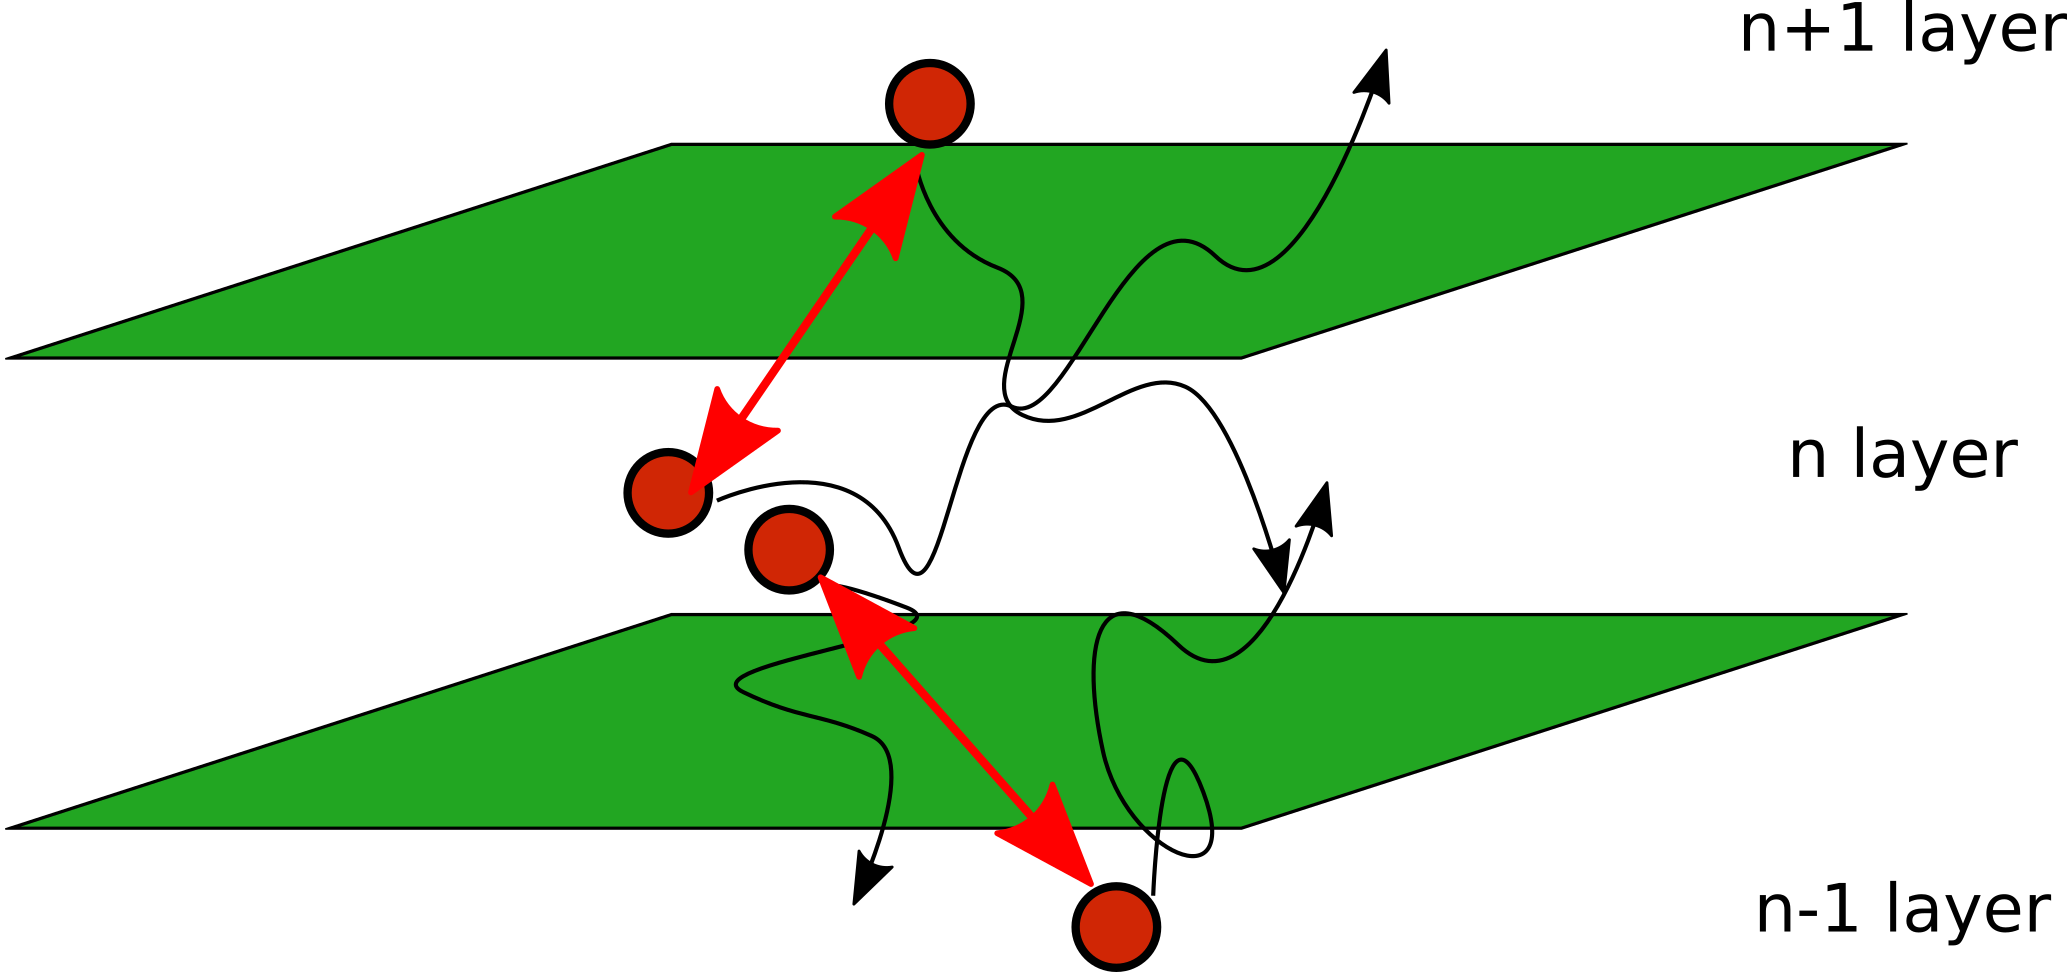
\includegraphics[width=\textwidth]{flow_layer.png}
				\begin{exampleblock}{ニュートン流体では}
					\begin{itemize}
						\item 隣接する粒子間の相互作用が、\alert{せん断速度やせん断応力に非依存。}
						\item 結果、粘度が一定。
						\item ただし、\alert{適正な範囲で。}
					\end{itemize}
				\end{exampleblock}
		\end{columns}
\end{frame}

\begin{frame}
    \frametitle{少しだけ大粒子が入った場合}
		\begin{itemize}
			\item ニュートン流体に球状粒子が入った場合。
				\begin{itemize}
					\item アインシュタインが理論的に導出
					\item 剛直な球を希薄に懸濁した溶液
				\end{itemize}
			\item 仮定条件
				\begin{itemize}
					\item 球の半径は、液体粒子より遥かに大きい。
					\item 球状粒子間の相互作用はない。
					\item 液体粒子は球状粒子に固着している。
				\end{itemize}
			\item 下式を使って、砂糖分子の大きさと分子数を概算
			\begin{itemize}
				\item 砂糖水の\alert{濃度と粘度との関係}から求めた。
			\end{itemize}
		\end{itemize}
		\begin{block}{アインシュタインの粘度式}
			\vspace{-5mm}
			\begin{align*}
				&\eta = \eta_0(1+2.5\phi) \\
				&\text{\small $\eta_0$は液体の粘度、$\phi$ は球状粒子の体積分率}
			\end{align*}
		\end{block}
\end{frame}

\begin{frame}
	\frametitle{アインシュタインの粘度式}
		\begin{center}
			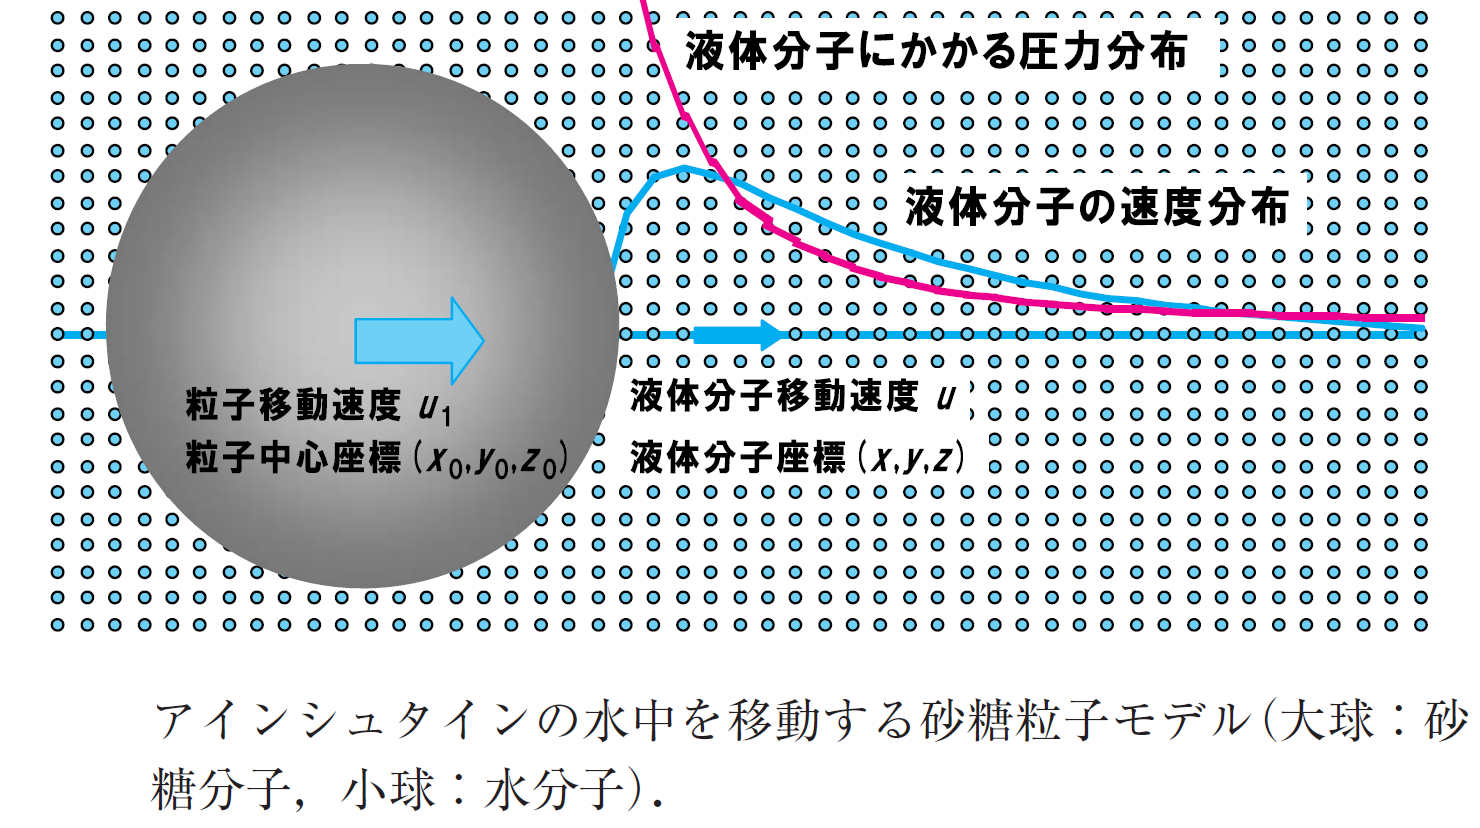
\includegraphics[width=.7\textwidth]{Einstein.png}
		\end{center}
		
		\begin{enumerate}
			\item すべての水分子の水平変位は、その相対位置を保ちながら起こる。
			\item 水分子の回転は、その相対位置を保ちながら起こる。
			\item 水の膨張・収縮は三次元で起こる。
		\end{enumerate}
\end{frame}

\section{非ニュートン流体}

\subsection{身近な液体とその分類}
\begin{frame}
	\frametitle{身近な液体}
		\begin{block}{身の回りにある各種の液体(流れるもの)の比較}
			\begin{columns}[T, onlytextwidth]
				\column{.48\linewidth}
					\begin{center}
						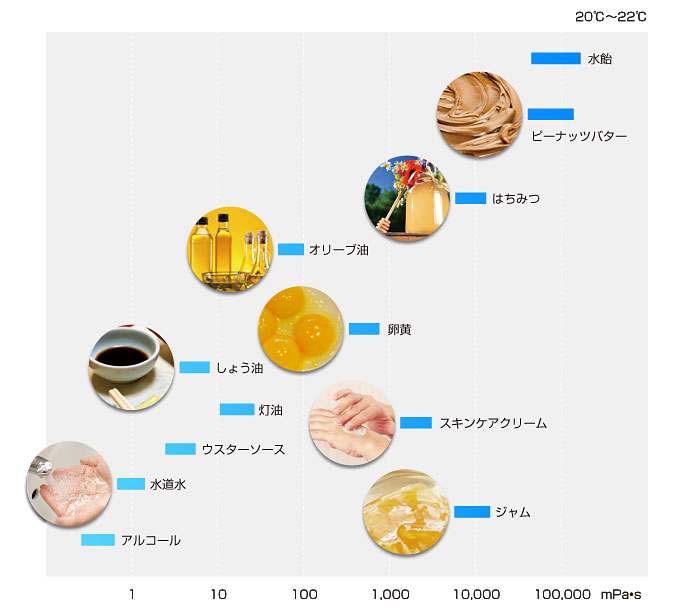
\includegraphics[width=\textwidth]{viscosity.jpg}
			
					\href{https://www.iwakipumps.jp/blog/naruhodo/08/}{この絵のサイトへのリンク}
					\end{center}
				\column{.48\linewidth}
					\begin{itemize}
						\item 一般的には左図のように、流れやすさを一覧に表す。
						\item 一応は、粘度の順番で並べて比較している。
						\item それで十分なのだろうか?
						\item<2> \alert{実は、測り方によっては順位は前後する場合も多い。}
					\end{itemize}
			\end{columns}
		\end{block}
\end{frame}

\begin{frame}
	\frametitle{各種の応答特性の分類}
		\begin{block}{ビンガム氏が作成した分類図}
			\begin{itemize}
				\item 図の左側が弾性応答で、右側が流動特性
				\item 単純に二分されるわけでもなく、粘性と弾性を\\併せ持ったものが多く存在。
			\end{itemize}
				\begin{center}
					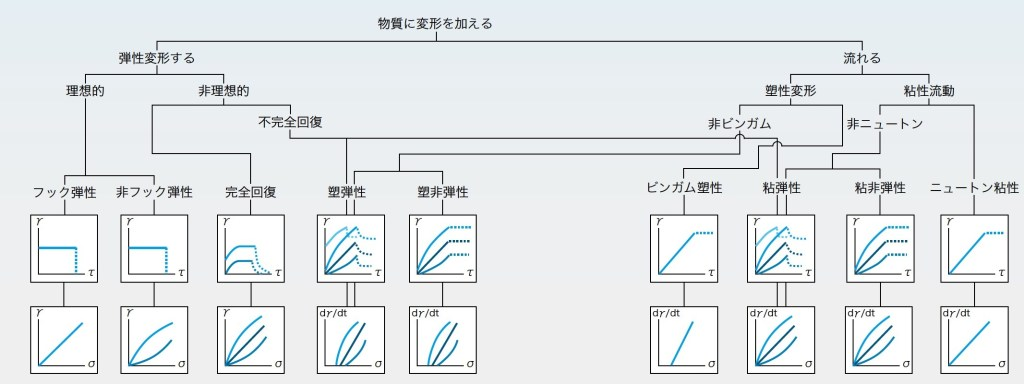
\includegraphics[width=.8\textwidth]{reoroji.jpeg}

					Nature 1942 v149-3790, p702

					\href{http://rheology.jp/nagoya/2017/10/レオロジー的な物質の分類/}{この絵のサイトへのリンク}
				\end{center}
		\end{block}
\end{frame}


\subsection{非ニュートン流体とは}
\begin{frame}
	\frametitle{非ニュートン流体とは}
		\begin{block}{非ニュートン流体とは?}
			\begin{itemize}
				\item 簡単に言えば、ニュートン流動と異なる流動特性を示すもの。
				\begin{itemize}
					\item ずり応力が線形ではない。
					\item 変形状態(ずり速度や加える力が変化)に依存して、粘度が変化する。
				\end{itemize}
				\item その原因は多数あるが、基本的に内部に構造を有する物質で生じる。
			\end{itemize}
		\end{block}
		\begin{columns}[T, onlytextwidth]
			\column{.48\linewidth}
				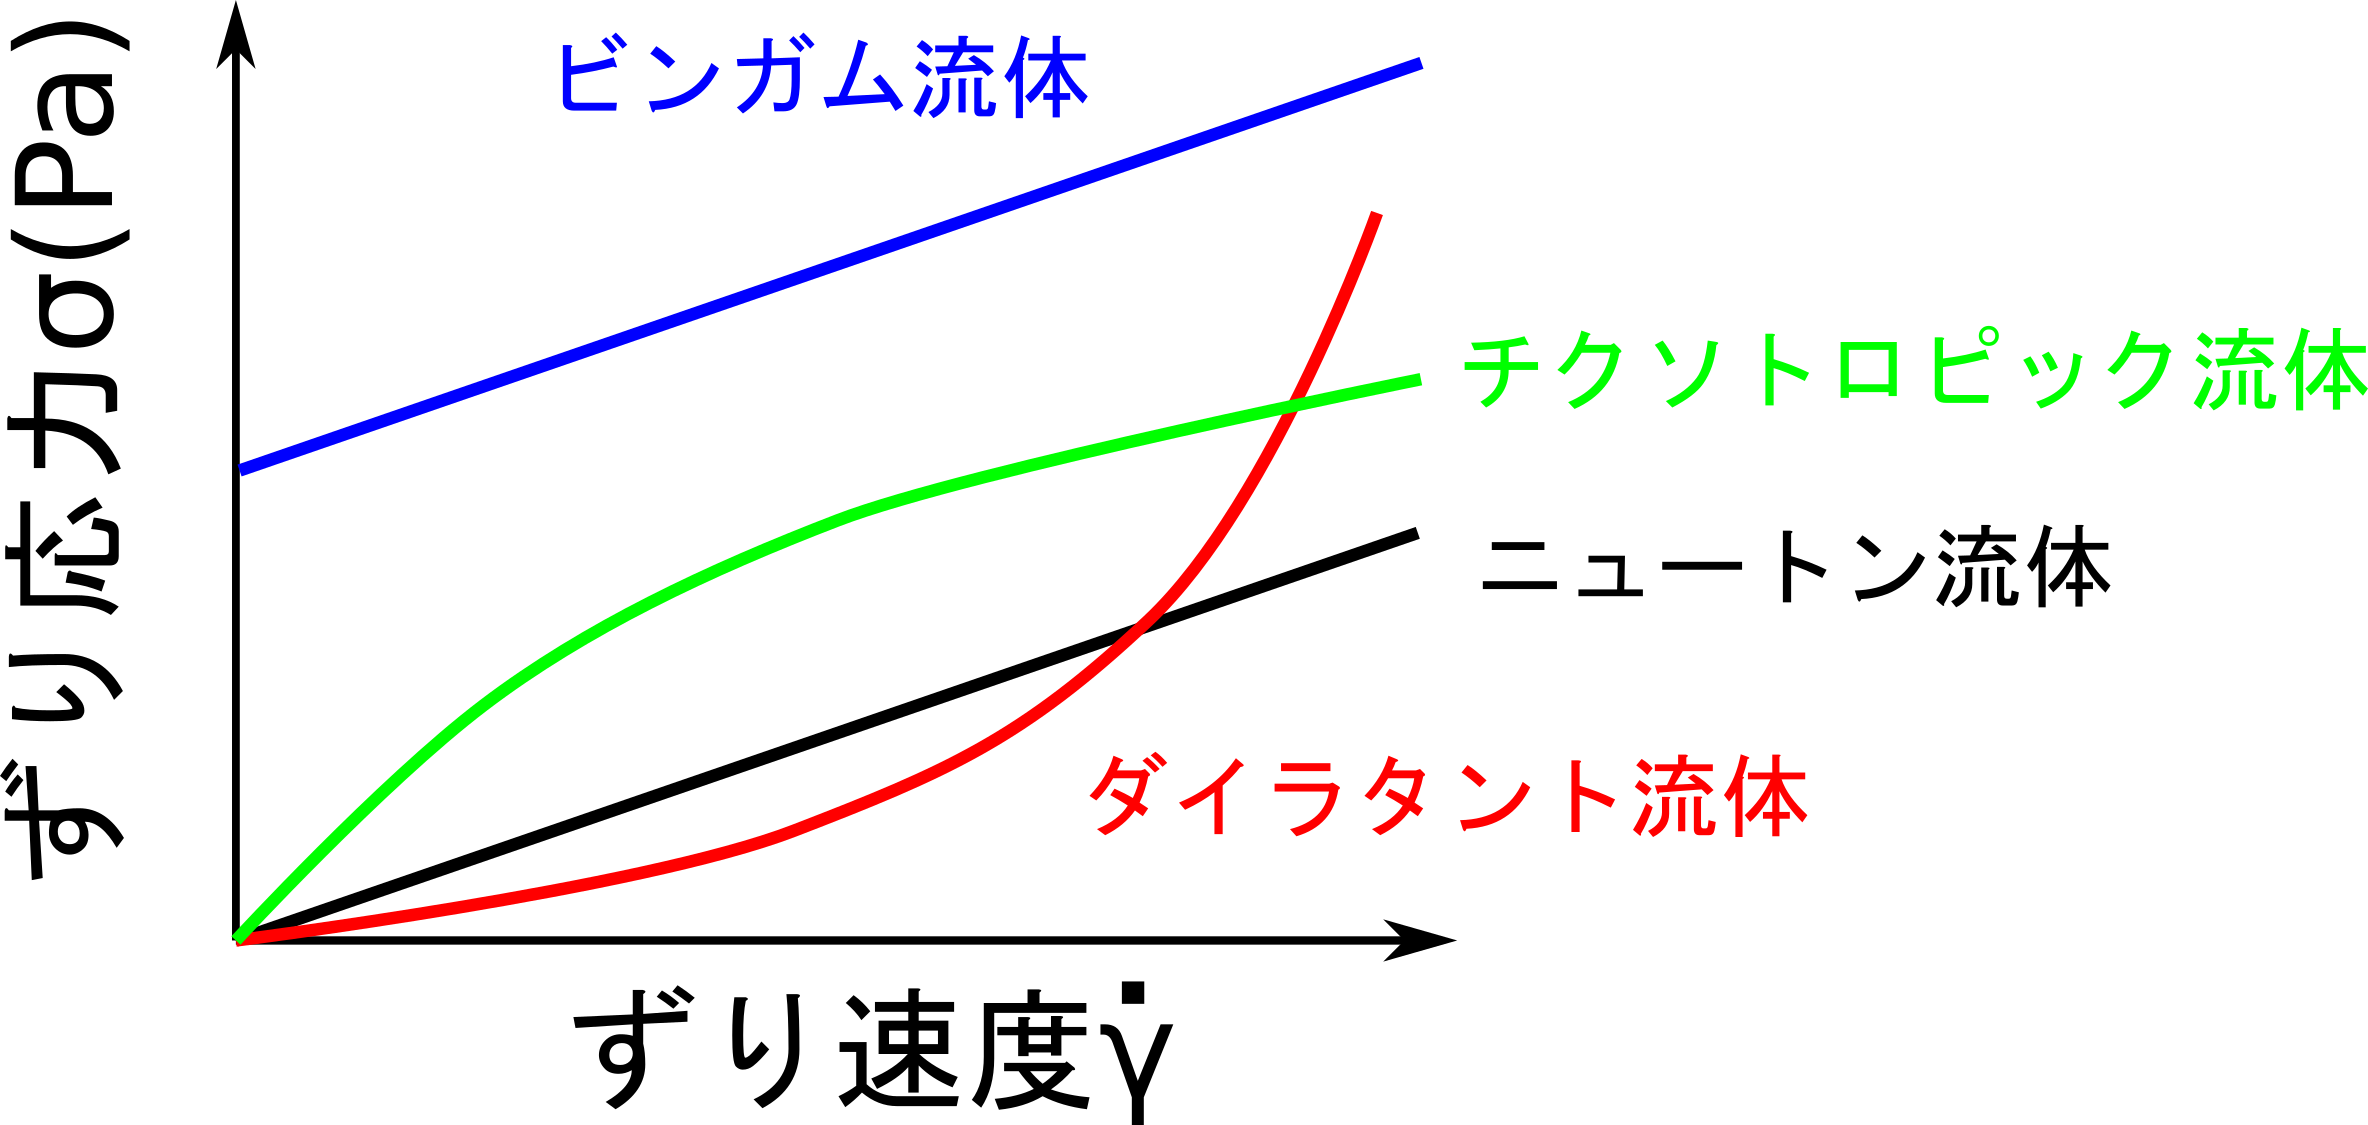
\includegraphics[width=\textwidth]{non_newtonian.png}
			\column{.48\linewidth}
				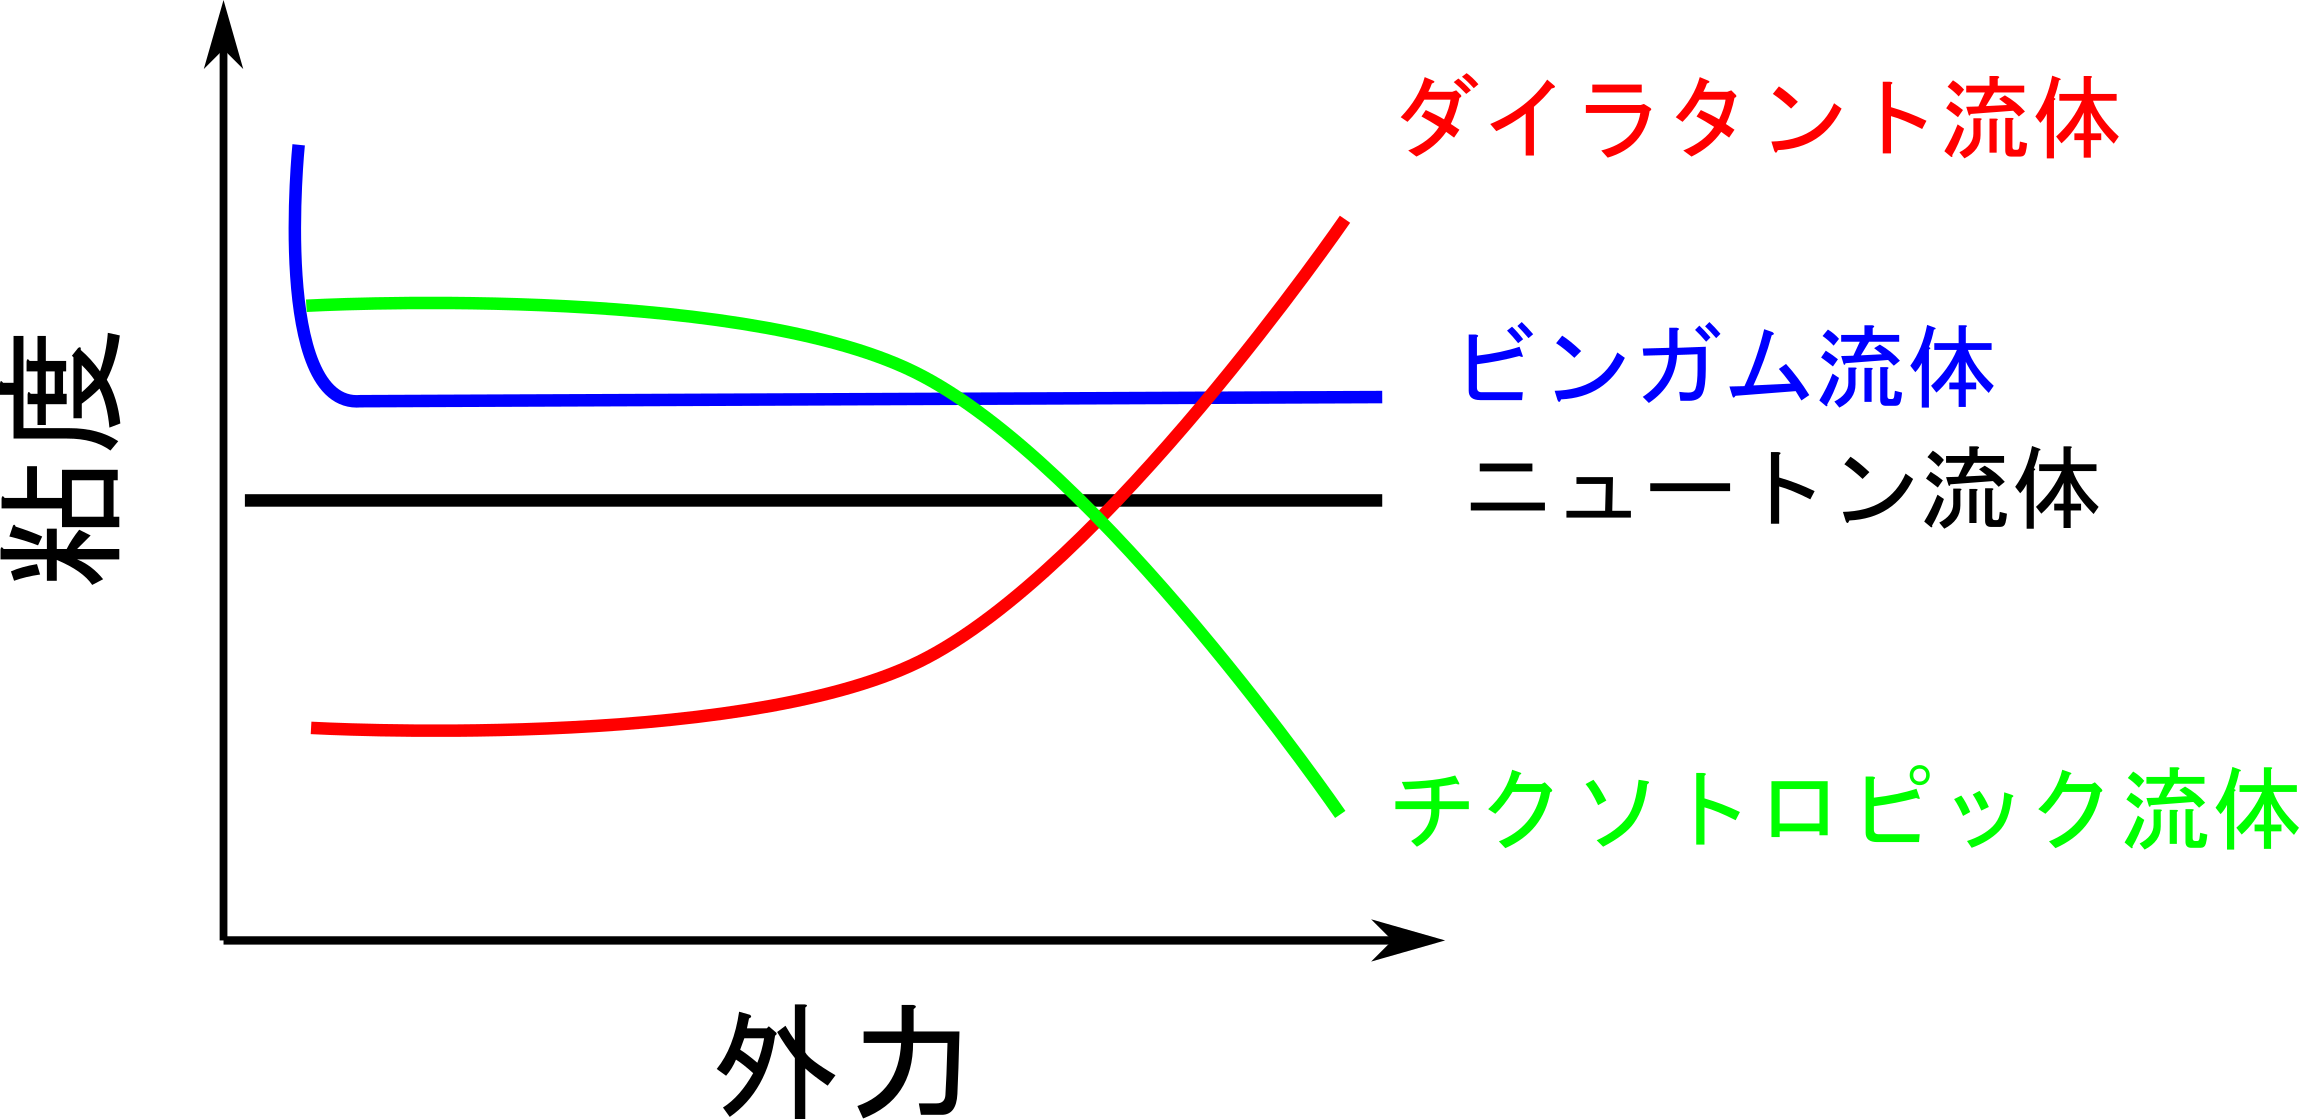
\includegraphics[width=\textwidth]{non_newtonian_2.png}				
		\end{columns}
\end{frame}

\subsection{非ニュートン性の発現}

\begin{frame}
	\frametitle{非ニュートン性の発現は?}
		\begin{block}{非ニュートン性発現の直感的理解}
			\begin{itemize}
				\item 物質の内部構造に由来して応力(粘度)が増加、減少
				\begin{itemize}
					\item 物質の内部構造に由来する特徴的時間が存在
					\item 内部構造が崩壊、再構築するための特徴的な時間
				\end{itemize}
				\item 外部からの変形に関わる時間(レート)との比が大事
				\begin{itemize}
					\item 物質中の内部構造が持つ特徴的な時間よりも短い時間(速い速度)で変形
					\begin{itemize}
						\item 内部構造が変化するため巨視的な粘度が変化
						\item \alert{非ニュートン性が発現}
					\end{itemize}
					\item 内部の特徴時間よりゆっくり変形
					\begin{itemize}
						\item その範囲では、粘度は変形速度に依存しない。
						\item ニュートニアンとして応答。
					\end{itemize}
				\end{itemize}
			\end{itemize}
		\end{block}
\end{frame}

\begin{frame}
	\frametitle{様々なせん断速度}
		以下に様々な工程における大体のせん断速度の範囲を、\\簡単にまとめた。
			\begin{center}
				\begin{tabular}{c|c} \hline
					工程 & せん断速度 \\ \hline \hline
					粒子の沈降	& $10^{-6} \sim 10^{-3}$ \\ \hline
					表面張力によるレベリング	& $10^{-2} \sim 10^{-1}$ \\ \hline
					重力による液垂れ	& $10^{-1} \sim 10^{1}$ \\ \hline \hline
					押し出し	& $10^{0} \sim 10^{3}$ \\ \hline
					ボトルからの流れ出し	& $10^{1} \sim 10^{2}$ \\ \hline
					噛む、飲む	& $10^{1} \sim 10^{2}$ \\ \hline
					混合攪拌	& $10^{1} \sim 10^{3}$ \\ \hline
					塗工	& $10^{0} \sim 10^{4}$ \\ \hline
				\end{tabular}
			\end{center}
\end{frame}

\section{実事象についても少しだけ考えましょう。}
\subsection{簡単な分類}
\begin{frame}
	\frametitle{シアシニングとシアシックニング}
		\begin{columns}[T, onlytextwidth]
			\column{.4\linewidth}
				\begin{center}
					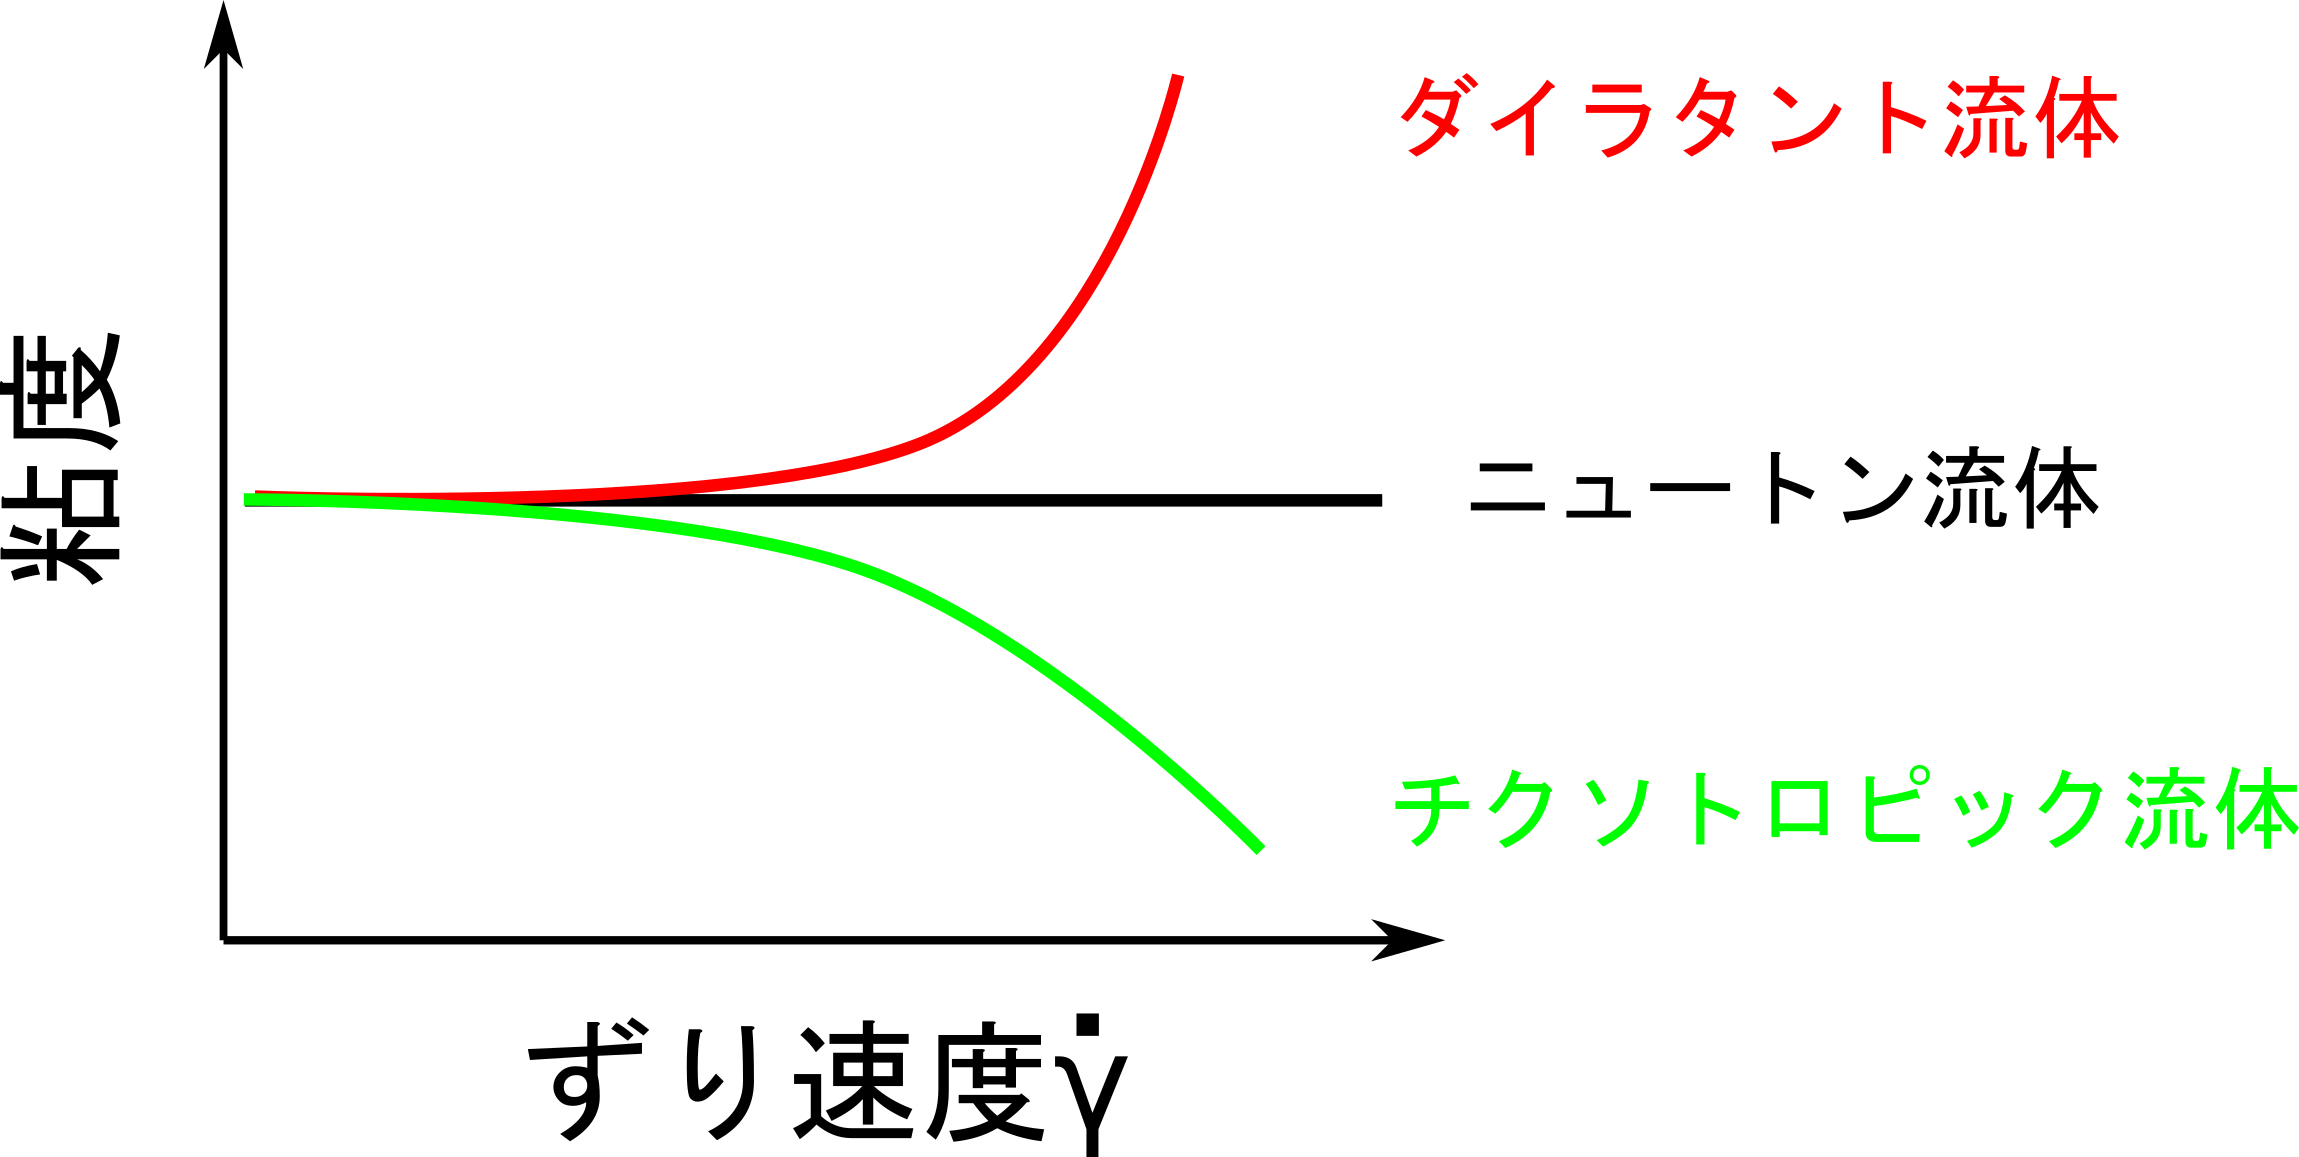
\includegraphics[width=1.1\textwidth]{non_newtonian_3.png}

					\vspace{10mm}
					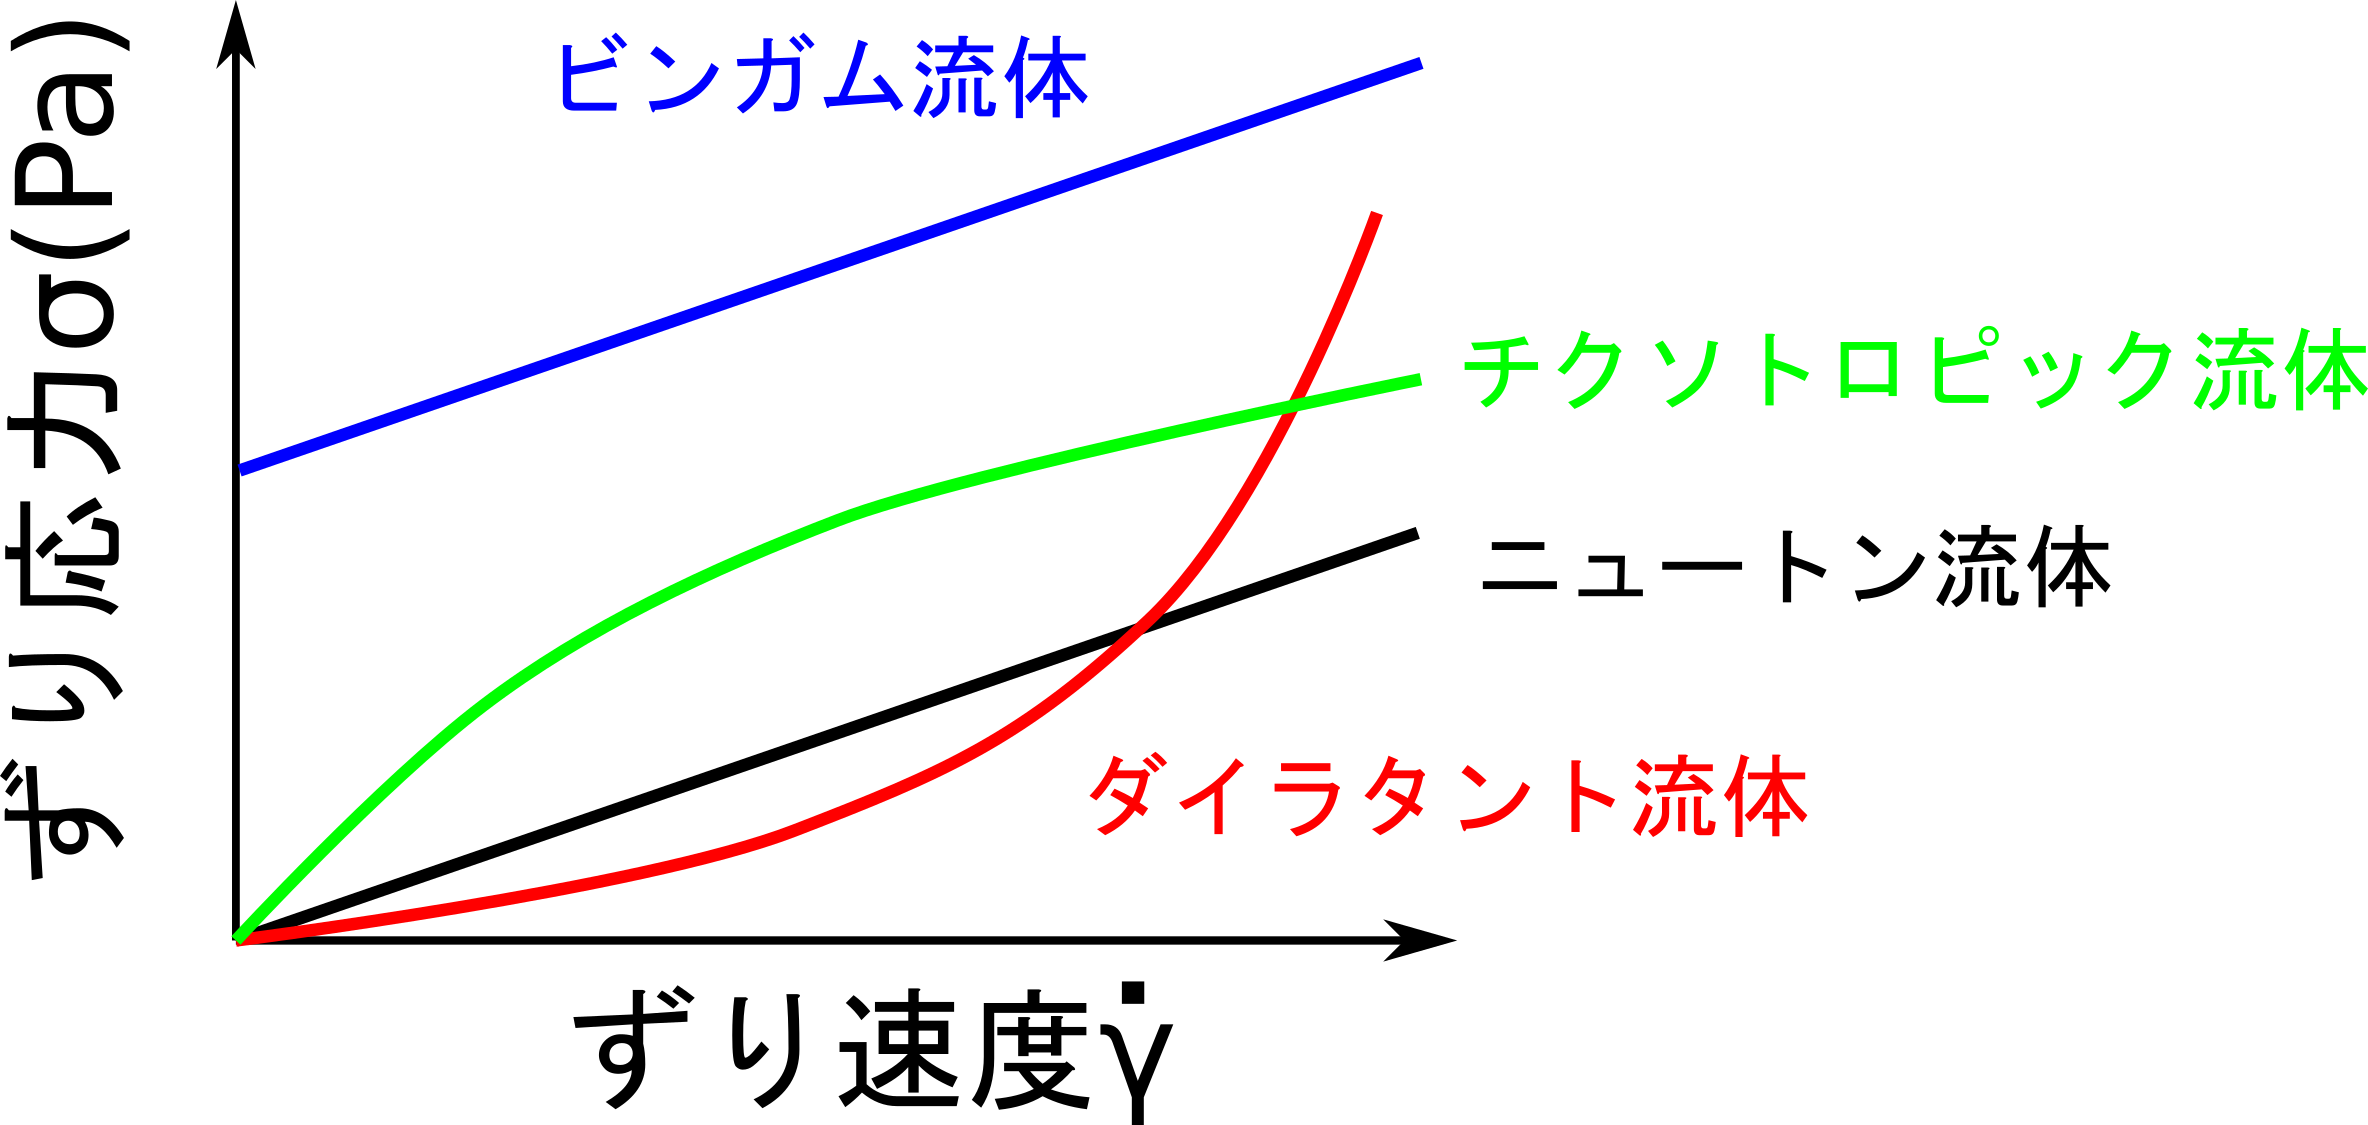
\includegraphics[width=1.1\textwidth]{non_newtonian.png}
				\end{center}
			\column{.56\linewidth}
				\begin{itemize}
					\item ひずみ速度の変化に対して、以下の2つに大まかに分類
					\begin{itemize}
						\item シア・シニング
						\begin{itemize}
							\item チクソトロピック流体
							\item ずり速度の増加により粘度が低下
						\end{itemize}
						\item シア・シックニング
						\begin{itemize}
							\item ダイラタント流体
							\item ずり速度の増加により粘度が上昇
						\end{itemize}
					\end{itemize}
					\item (参考)ニュートン流体
						\begin{itemize}
							\item 粘度がずり速度に依存しない。
							\item ずり速度が上がれば、応力は増加することに注意。
						\end{itemize}
				\end{itemize}
			\end{columns}
\end{frame}


\subsection{シアシニングについて}
\begin{frame}
	\frametitle{シアシニングについて}
			\begin{columns}[T, onlytextwidth]
				\column{.5\linewidth}
				\begin{exampleblock}{シア・シニングの挙動}
					\begin{itemize}
						\item 静置状態では内部構造が形成されて高粘度。
						\item 高せん断速度が付与されることで、
						\begin{itemize}
							\item 内部構造が崩壊して粘度が低下。
						\end{itemize}
						\item せん断速度の低下により、粘度が再上昇。
					\end{itemize}
				\end{exampleblock}
				\column{.4\linewidth}
					\begin{center}
						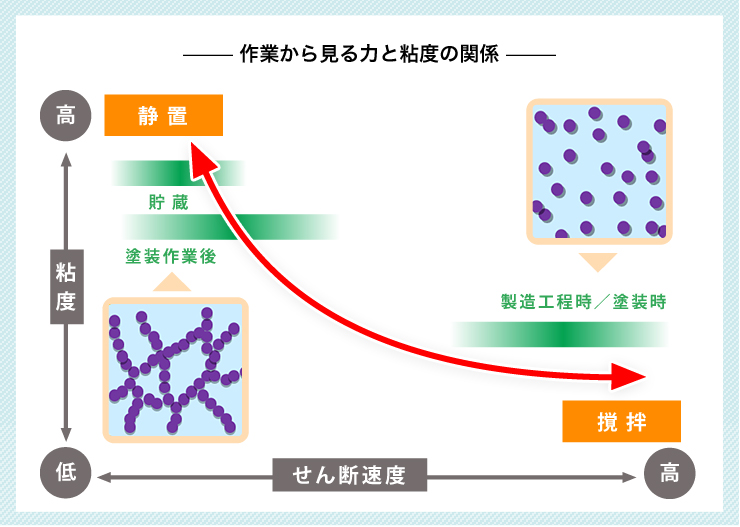
\includegraphics[width=1.2\textwidth]{thixotropy_1w.jpg}
				
						\href{https://www.kyoeisha.co.jp/product/toryou/antisaggingagentTechnology.php}{この画像のサイト}
					\end{center}
			\end{columns}
		
\end{frame}

\begin{frame}
	\frametitle{塗膜の液垂れ防止}
			\begin{columns}[T, onlytextwidth]
				\column{.5\linewidth}
					\begin{block}{塗膜の液垂れ}
						\begin{itemize}
							\item 塗布後に、
							% \begin{itemize}
								\item 内部構造の再形成が遅くて、
								\item 塗料の粘度が低すぎた場合、
							% \end{itemize}
							\item 塗膜の液垂れ発生
						\end{itemize}
					\end{block}
				\column{.4\linewidth}
					\begin{center}
						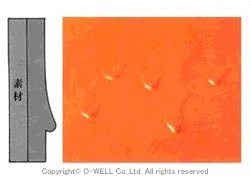
\includegraphics[width=1.2\textwidth]{ekidare.jpg}
		
						\href{http://www.owell.co.jp/knowlegde/trouble/ta004.html}{この画像のサイト}
					\end{center}
			\end{columns}
			% このような挙動は、例えば、塗装工程等で重要であり、この特性を上手に設計することで塗膜の液垂れを防止することができるようになります。
			\begin{alertblock}{設計のポイント}
				具体的には、生地状態に復帰したときの内部構造の再構築に必要な特徴的な時間を短くすることが大事になります。
			\end{alertblock}
\end{frame}

\begin{frame}
	\frametitle{ビンガム流体}
		\begin{center}
			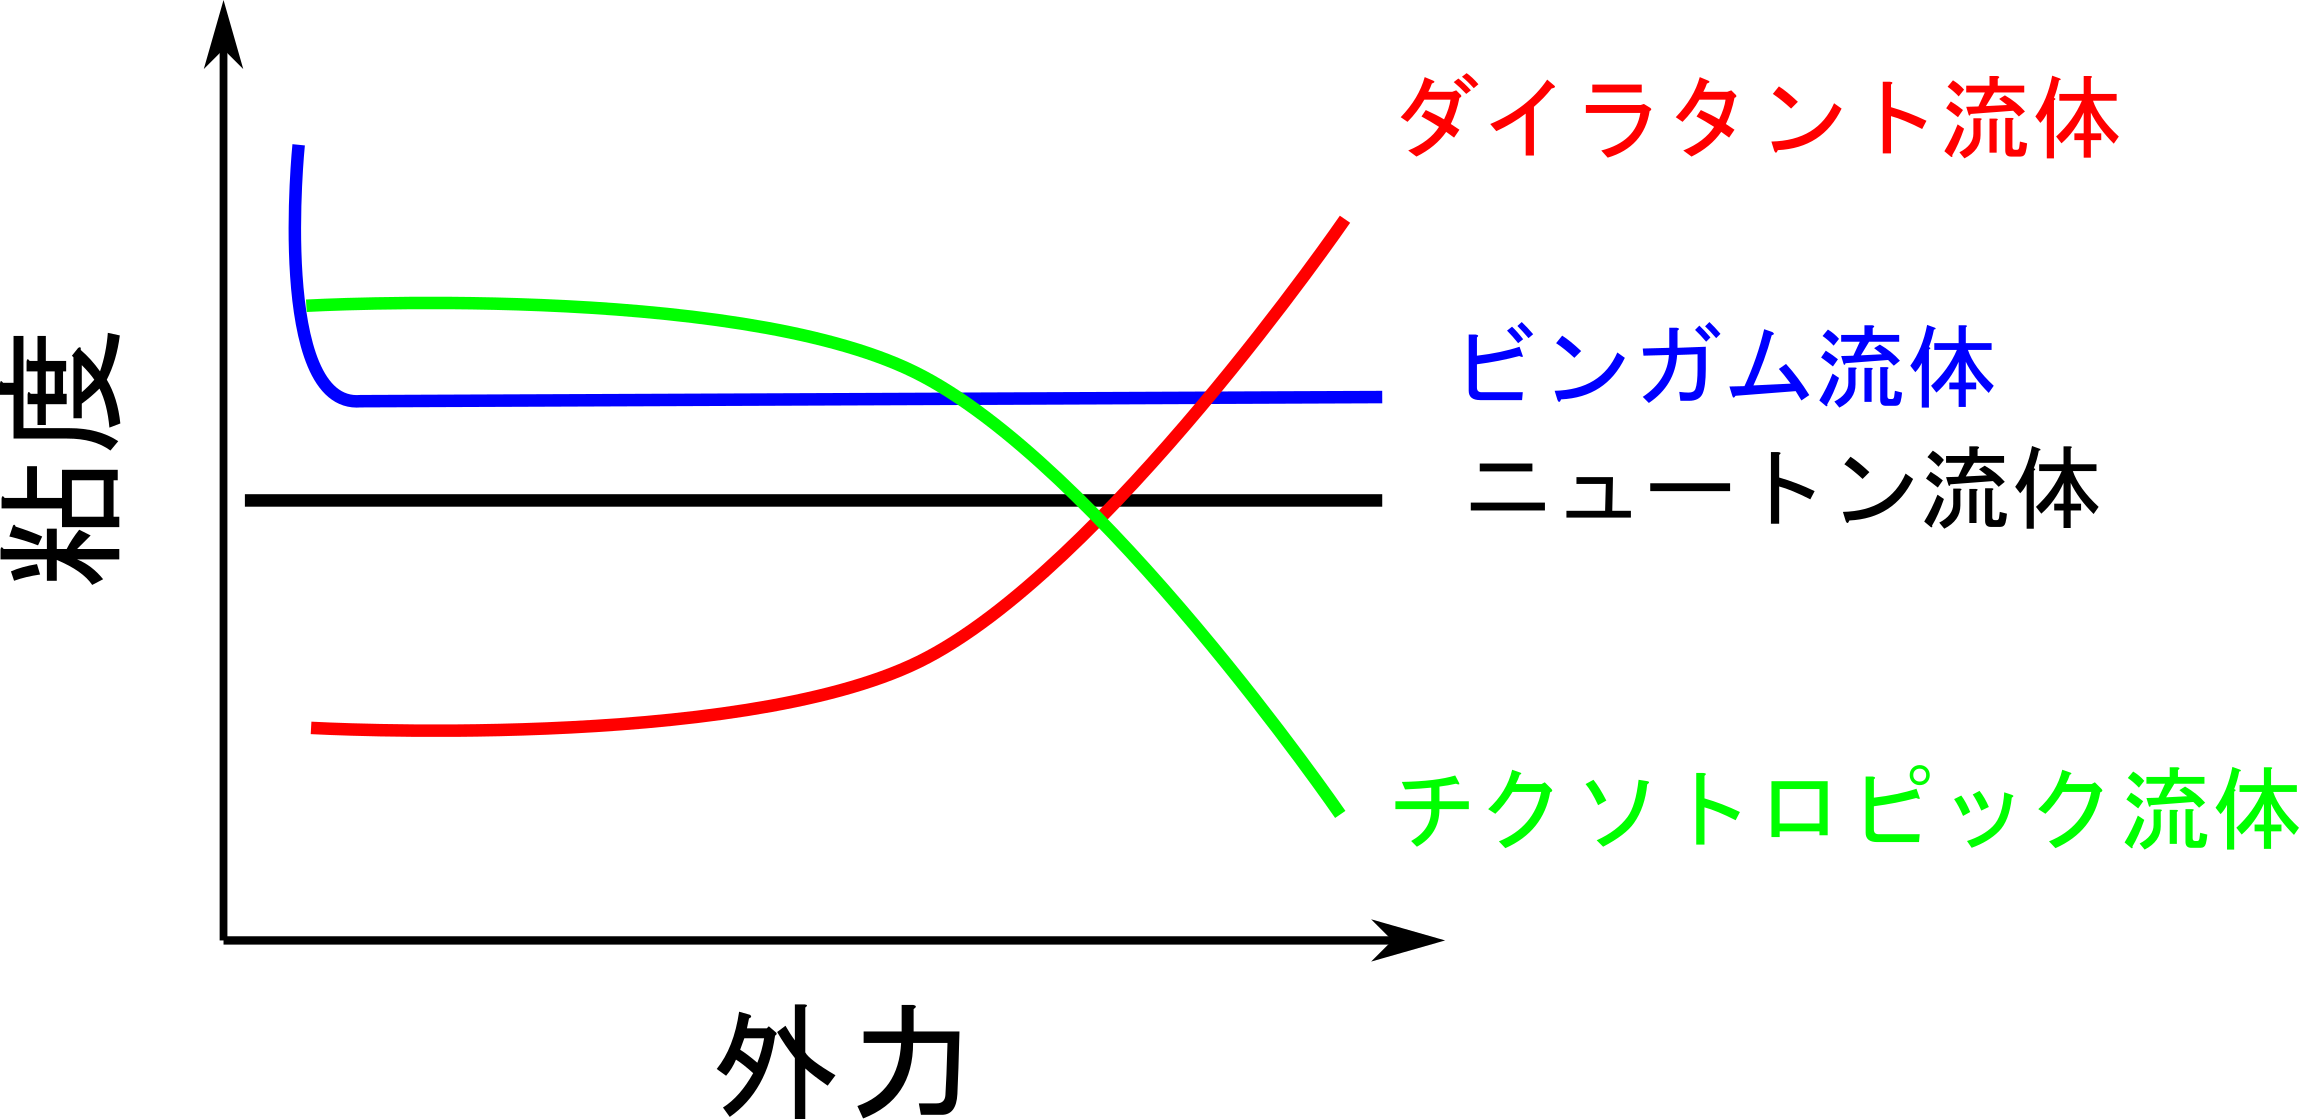
\includegraphics[width=.6\textwidth]{non_newtonian_2.png}
		\end{center}
		\begin{itemize}
			\item 降伏値を有する流体
			\begin{itemize}
				\item ある一定の力がかかるまでは固体。
				\item 降伏値を超えると流動
			\end{itemize}
			\item チクソトロピック流体とほぼ類似の挙動
			\begin{itemize}
				\item 内部構造が一旦崩壊すると、相互作用が一気に小さく。
			\end{itemize}
			\item 実例
			\begin{itemize}
				\item バター
				\item 歯磨き粉
			\end{itemize}
		\end{itemize}
\end{frame}

\subsection{シアシックニングについて}
\begin{frame}
	\frametitle{ダイラタンシーについて}
		\begin{center}
			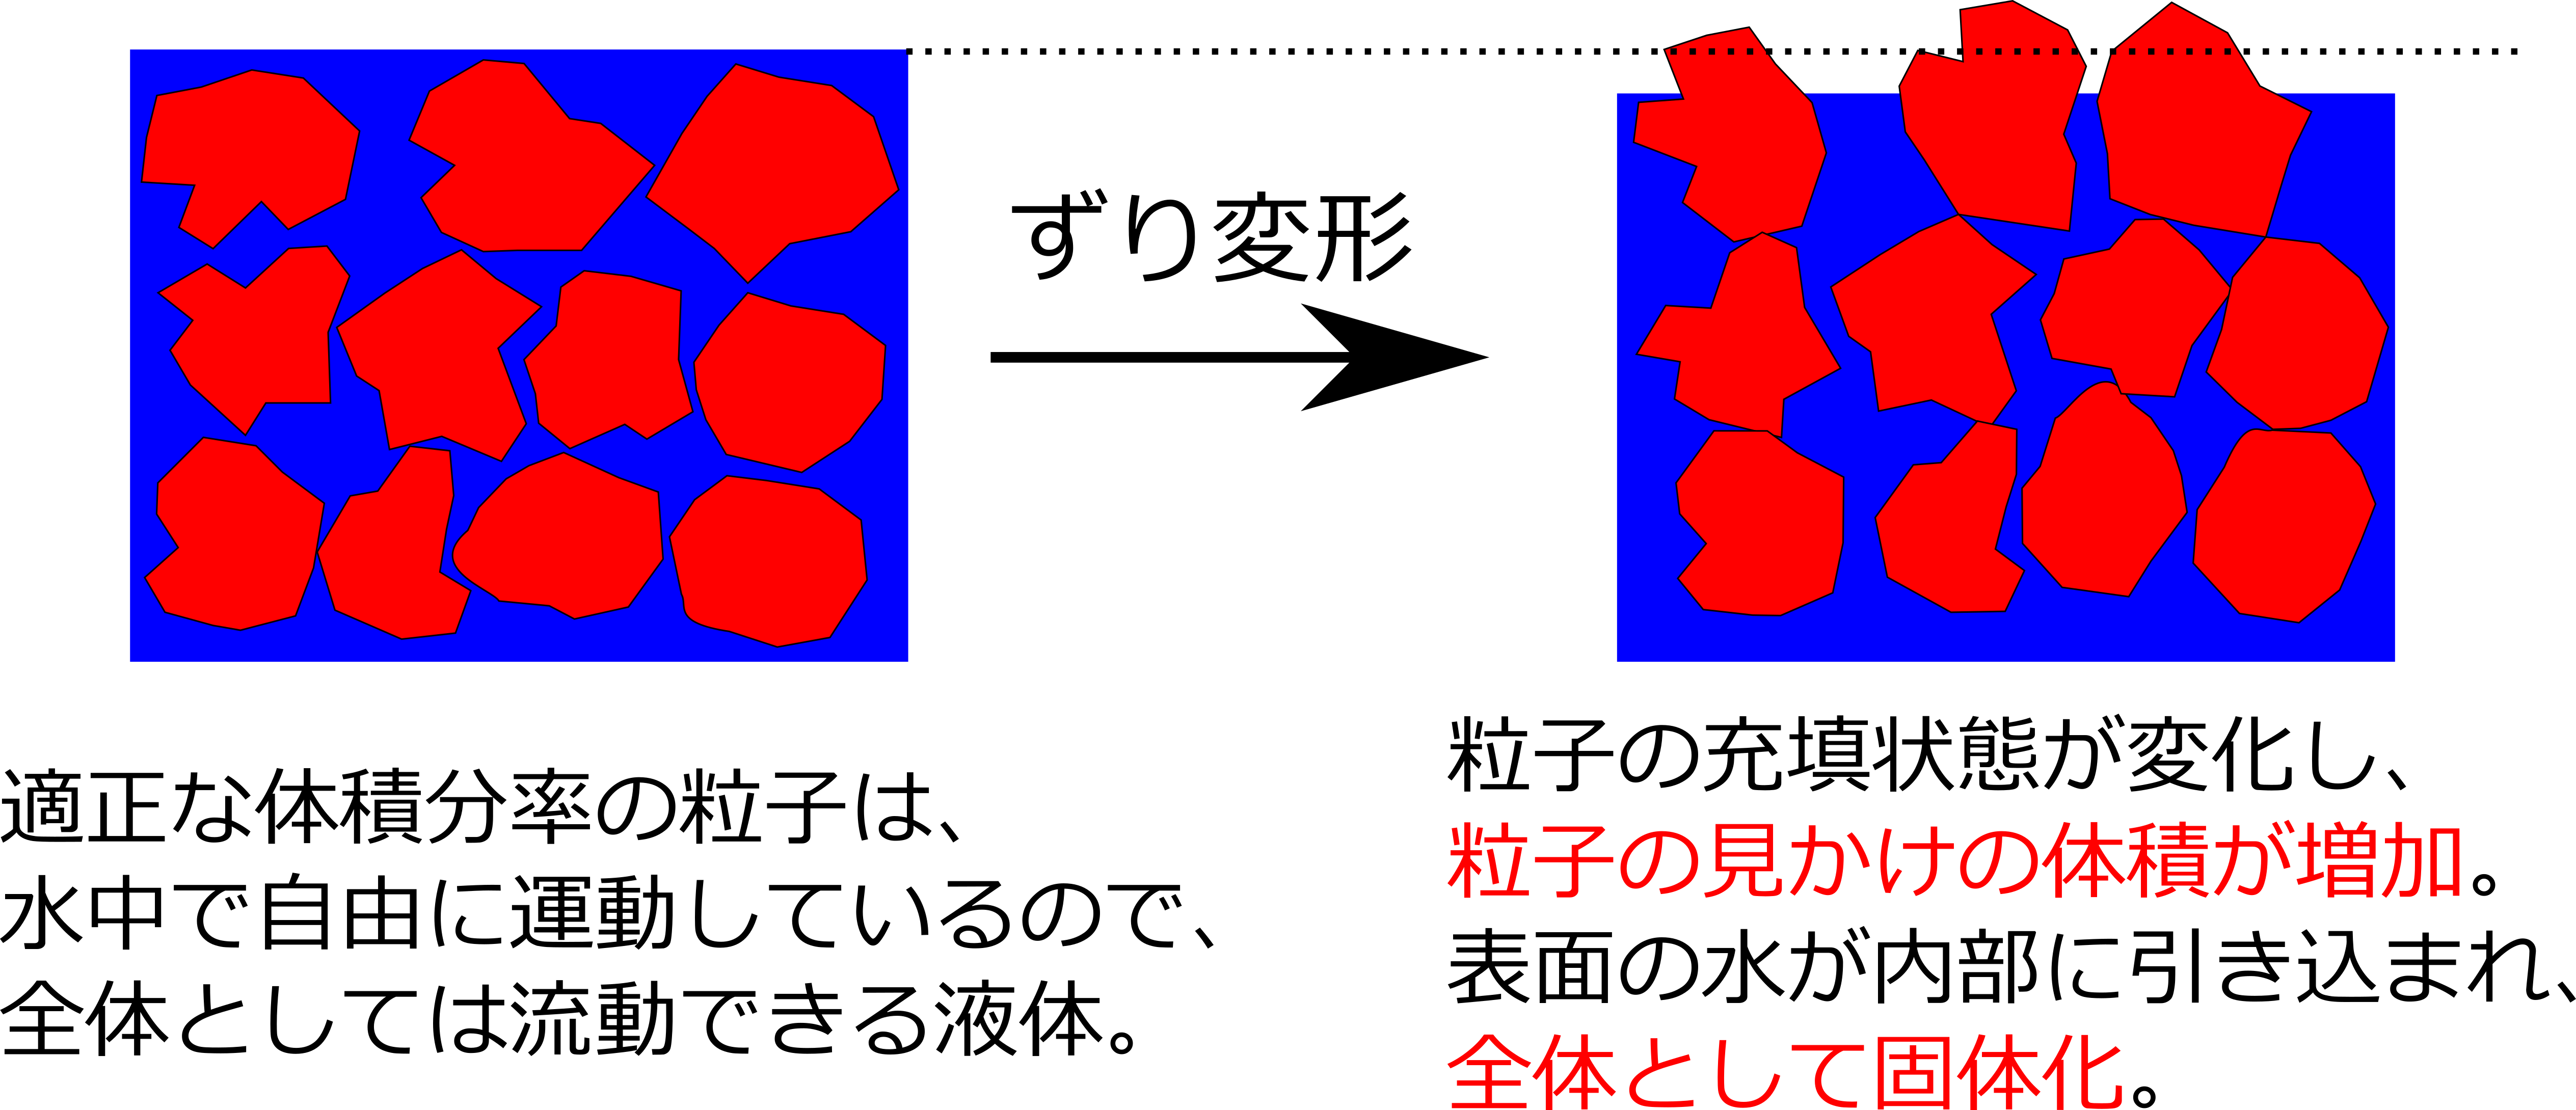
\includegraphics[width=.8\textwidth]{dilatancy.png}
		\end{center}
		\small
		\begin{itemize}
			\item おなじ大きさの球形粒子の水を吸った状態を考える。
			\item 最密充填では空隙率は26%で、これ以上の水があれば流動。
			\item 急激な外力により単純立方格子になると空隙率は48%になるため、水は全部内部へ吸いこまれる。
			\item こすり合う粒子ができて体積が幾分膨張、もろい固体となる。
		\end{itemize}
\end{frame}

% \begin{frame}
% 	\frametitle{実事象でのダイラタンシー}

% 	\begin{columns}[T, onlytextwidth]
% 		\column{.46\linewidth}
% 			\begin{itemize}
% 				\item \href{https://youtu.be/cnhgilMWdv0}{ニュートン流体と比較}
% 				\vspace{3mm}
% 				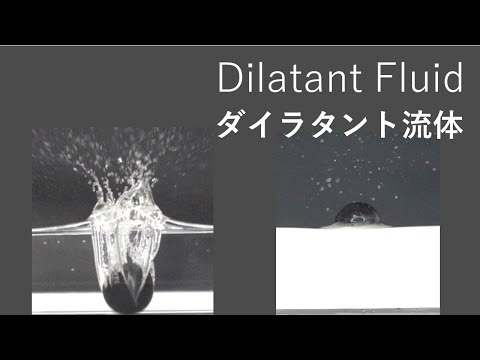
\includegraphics[width=.6\textwidth]{dilatant_youtube.jpg}

% 				% https://img.youtube.com/vi/cnhgilMWdv0/hqdefault.jpg

% 				\item 車で走れる砂浜
% 				\vspace{-5mm}
% 				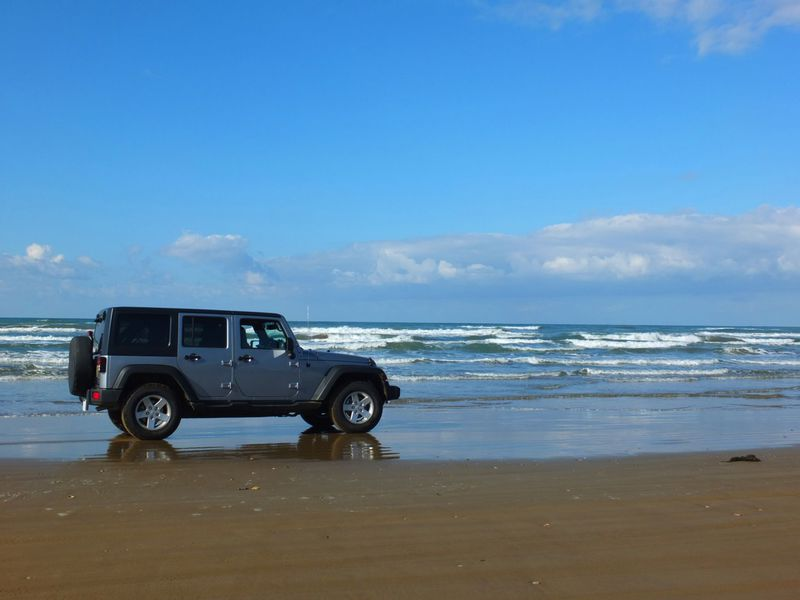
\includegraphics[width=.6\textwidth]{senrihama.jpg}
% 			\end{itemize}
% 		\column{.46\linewidth}
% 			\begin{itemize}
% 				\item 工業的利用の可能性
% 				\href{https://youtu.be/L5Ts9lYZIDk}{「リキッドアーマー」}
% 				\vspace{3mm}
% 				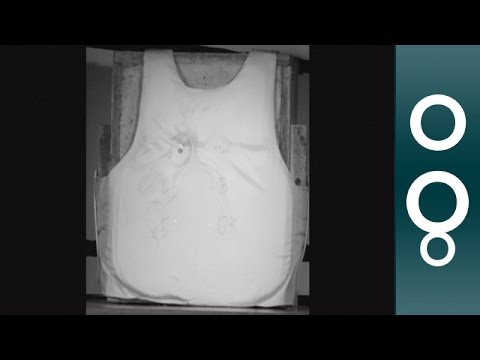
\includegraphics[width=.6\textwidth]{liquid_armour.jpg}
% 				\begin{itemize}
% 					\item 防弾チョッキ等への応用も検討
% 					\item ケブラーに充填液を含浸
% 					\item 未だ実用化には至っていない
% 				\end{itemize}
% 			\end{itemize}
% 	\end{columns}
% \end{frame}

\begin{frame}
	\frametitle{おまけ}
		\begin{columns}[T, onlytextwidth]
			\column{.48\linewidth}
				\begin{center}
					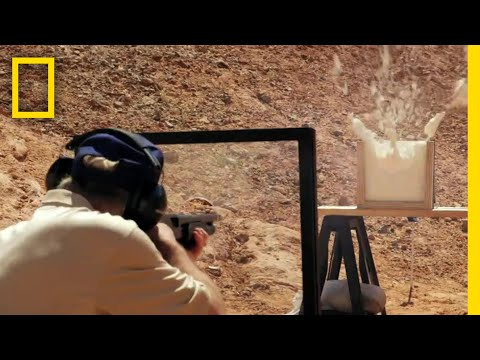
\includegraphics[width=\textwidth]{sweets.jpg}

					\href{https://www.youtube.com/watch?v=wKZDOLWjd7Y}{スイーツとダイラタンシー}
				\end{center}
			\column{.48\linewidth}
				\begin{center}
					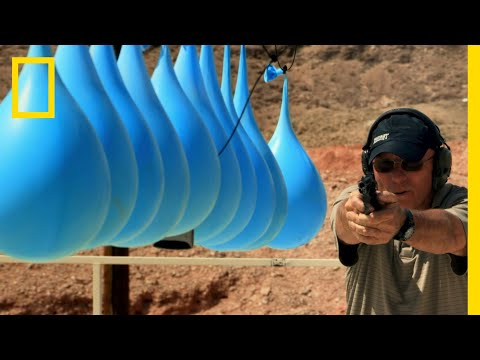
\includegraphics[width=\textwidth]{baloon.jpg}

					\href{https://www.youtube.com/watch?v=kRLJti62CGE}{水によるエネルギー散逸}
				\end{center}
		\end{columns}
	

	
\end{frame}


% \appendix
% \backupbegin

% % \section{演習問題 1}
% % \subsection{「物質の三態について」}
% % \begin{frame}
% % 	\frametitle{「物質の三態について」}
% % 	\scriptsize
% % 	以下の穴を埋めてください。
% % 		\begin{itemize}
% % 			\item 関数の役割を考えてみると、\fbox{\textcolor{red}{入力}}を変換装置に入れた結果として\fbox{\textcolor{red}{出力}}が現れるわけですから、入力と出力との間の\fbox{\textcolor{red}{関係}}を表していると考えることもできます。
% % 			\item また、関数というのは、\fbox{\textcolor{red}{数の集合}}に値を取る\fbox{\textcolor{red}{写像}}の一種と考えることもできます。
% % 			\item グラフとは、\fbox{\textcolor{red}{入力}}と\fbox{\textcolor{red}{出力}}との関係を\fbox{\textcolor{red}{平面図}}に示したものであり、視覚的にその関係を理解しやすくしたものと考えることができます。
% % 			\item このグラフに表した関数の\fbox{\textcolor{red}{形}}を見ることで、入力と出力との\fbox{\textcolor{red}{関係}}を直感的に理解することができます。
% % 		\end{itemize}
% % \end{frame}

% \backupend
\end{document}